%%%%%%%%%%%%%%%%%%%%%%%%%%%%%%%%%%%%%%%%%%%%%%%%%%%%%%%%%%%%%%%%%%%%%%%%%
%  Zawartość: Główny plik szablonu pracy dyplomowej (magisterskiej/inżynierskiej).
%  Opracował: Tomasz Kubik <tomasz.kubik@pwr.edu.pl>
%  Data: kwiecień 2016
%  Wersja: 0.2
%%%%%%%%%%%%%%%%%%%%%%%%%%%%%%%%%%%%%%%%%%%%%%%%%%%%%%%%%%%%%%%%%%%%%%%%%

\documentclass[a4paper,onecolumn,oneside,12pt,extrafontsizes]{memoir}
% W celu przygotowania wydruku do archiwum należy przesłonić komendę powyższą
% dwoma poniższymi komendami:
%\documentclass[a4paper,onecolumn,twoside,10pt]{memoir} 
%\renewcommand{\normalsize}{\fontsize{8pt}{10pt}\selectfont}

%\usepackage[cp1250]{inputenc} % jeśli kodowanie edytowanych plików to cp1250 
\usepackage[utf8]{inputenc} % jeśli kodowanie edytowanych plików to UTF8
\usepackage[T1]{fontenc}
\usepackage[polish]{babel}
%\DisemulatePackage{setspace}
\usepackage{setspace}
\usepackage{tabularx}
\usepackage{color,calc}
%\usepackage{soul} % pakiet z komendami do podkreślania tekstu

\usepackage{ebgaramond} % pakiet z czcionkami garamond, potrzebny tylko do strony tytułowej, musi wystąpić przed pakietem tgtermes

%% Aby uzyskać polskie literki w pdfie (a nie zlepki) korzystamy z pakietu czcionek tgterms. 
%% W pakiecie tym są zdefiniowane klony czcionek Times o kształtach: normalny, pogrubiony, italic, italic pogrubiony.
%% W pakiecie tym brakuje czcionki o kształcie: slanted (podobny do italic). 
%% Jeśli w dokumencie gdzieś zostanie zastosowana czcionka slanted (np. po użyciu komendy \textsl{}), to
%% latex dokona podstawienia na czcionkę standardową i zgłosi to w ostrzeżeniu (warningu).
%% Ponadto tgtermes to czcionka do tekstu. Wszelkie matematyczne wzory będą sformatowane domyślną czcionką do wzorów.
%% Jeśli wzory mają być sformatowane z wykorzystaniem innych czcionek, trzeba to jawnie zadeklarować.

%% Po zainstalowaniu pakietu tgtermes może będzie trzeba zauktualizować informacje 
%% o dostępnych fontach oraz mapy. Można to zrobić z konsoli (jako administrator)
%% initexmf --admin --update-fndb
%% initexmf --admin --mkmaps

\usepackage{tgtermes}   
\renewcommand*\ttdefault{txtt}

% We wcześniejszej wersji szablonu korzystano z innych czcionek. Dla celów historycznych pozostawiono je w komentarzu
%\usepackage{mathptmx} % pakiet będący następcą pakietów times and mathptm, niestety polskie literki są zlepkami
%\usepackage{newtxtext,newtxmath} % pakiety dostarczające Times dla tekstów i wzorów matematycznych,  
%                                  rozwiązuje problemy występujące w mathptmx, ale wymaga zainstalowania
%                                  dodatkowych pakietów oraz uruchomienia updmap (konsola administratora)
%                                  niestety polskie literki są zlepkami
%\usepackage{newtxmath,tgtermes} % można też połączyć czcionki do tekstu i czcionki do wzorów

\usepackage{listings} % pakiet do prezentacji kodu. 
\renewcommand{\lstlistingname}{Kod źródłowy}
\definecolor{light-gray}{gray}{0.5}
%Wcześniej był problem z polskimi znakami w otoczeniu lstlisting, stąd pozostawiono w komentarzu zastosowane wtedy rozwiązanie: 
\lstset{
  %commentstyle=\color{dkgreen},
  breaklines=true,
  postbreak=\mbox{\textcolor{red}{$\hookrightarrow$}\space},
  numbers=left,
  showtabs=false,
  breakatwhitespace=true,
  basicstyle=\ttfamily\small,
  columns=fullflexible,
  showstringspaces=false,
  showspaces=false,
  xleftmargin=3em,
  framexleftmargin=2.5em,
  frame=tb,
  breaklines=true,
  framextopmargin=5pt,
  framexbottommargin=7pt,
  commentstyle=\color{light-gray}\upshape
%  inputencoding=utf8x, 
  extendedchars=\true,
  literate={ą}{{\k{a}}}1
             {Ą}{{\k{A}}}1
             {ę}{{\k{e}}}1
             {Ę}{{\k{E}}}1
             {ó}{{\'o}}1
             {Ó}{{\'O}}1
             {ś}{{\'s}}1
             {Ś}{{\'S}}1
             {ł}{{\l{}}}1
             {Ł}{{\L{}}}1
             {ż}{{\.z}}1
             {Ż}{{\.Z}}1
             {ź}{{\'z}}1
             {Ź}{{\'Z}}1
             {ć}{{\'c}}1
             {Ć}{{\'C}}1
             {ń}{{\'n}}1
             {Ń}{{\'N}}1                            
}

% Choć możliwe jest zastosowanie różnych pakietów formatujących tabele, zaleca się tego nie robić.
%\usepackage{longtable}
%\usepackage{ltxtable}
%\usepackage{tabulary}

%%%%%%%%%%%%%%%%%%%%%%%%%%%%%%%%%%%%%%%%%%%%%%%%%%%
%% Ustawienia odpowiedzialne za sposób łamania dokumentu
%% i ułożenie elementów pływających
%%%%%%%%%%%%%%%%%%%%%%%%%%%%%%%%%%%%%%%%%%%%%%%%%%%
%\hyphenpenalty=10000		% nie dziel wyrazów zbyt często
\clubpenalty=10000      %kara za sierotki
\widowpenalty=10000  % nie pozostawiaj wdów
\brokenpenalty=10000		% nie dziel wyrazów między stronami
\exhyphenpenalty=999999		% nie dziel słów z myślnikiem
\righthyphenmin=3			% dziel minimum 3 litery

%\tolerance=4500
%\pretolerance=250
%\hfuzz=1.5pt
%\hbadness=1450

\renewcommand{\topfraction}{0.95}
\renewcommand{\bottomfraction}{0.95}
\renewcommand{\textfraction}{0.05}
\renewcommand{\floatpagefraction}{0.35}

%%%%%%%%%%%%%%%%%%%%%%%%%%%%%%%%%%%%%%%%%%%%%%%%%%%
%%  Ustawienia rozmiarów: tekstu, nagłówka i stopki, marginesów
%%  dla dokumentów klasy memoir 
%%%%%%%%%%%%%%%%%%%%%%%%%%%%%%%%%%%%%%%%%%%%%%%%%%%
\setlength{\headsep}{10pt} 
\setlength{\headheight}{13.6pt} % wartość baselineskip dla czcionki 11pt tj. \small wynosi 13.6pt
\setlength{\footskip}{\headsep+\headheight}
\setlength{\uppermargin}{\headheight+\headsep+1cm}
\setlength{\textheight}{\paperheight-\uppermargin-\footskip-1.5cm}
\setlength{\textwidth}{\paperwidth-6cm}
\setlength{\spinemargin}{3.5cm}
\setlength{\foremargin}{2.5cm}
\setlength{\marginparsep}{2mm}
\setlength{\marginparwidth}{2.3mm}
%\settrimmedsize{297mm}{210mm}{*}
%\settrims{0mm}{0mm}	
\checkandfixthelayout[fixed] % konieczne, aby się dobrze wszystko poustawiało
%%%%%%%%%%%%%%%%%%%%%%%%%%%%%%%%%%%%%%%%%%%%%%%%
%%  Ustawienia odległości linii, wcięć, odstępów
%%%%%%%%%%%%%%%%%%%%%%%%%%%%%%%%%%%%%%%%%%%%%%%%
%\linespread{1.5}
\linespread{1.241}
\setlength{\parindent}{14.5pt}
%\setbeforesecskip{10pt plus 0.5ex}%{-3.5ex \@plus -1ex \@minus -.2ex}
%\setaftersecskip{10pt plus 0.5ex}%\onelineskip}
%\setbeforesubsecskip{8pt plus 0.5ex}%{-3.5ex \@plus -1ex \@minus -.2ex}
%\setaftersubsecskip{8pt plus 0.5ex}%\onelineskip}
%\setlength\floatsep{6pt plus 2pt minus 2pt} 
%\setlength\intextsep{12pt plus 2pt minus 2pt} 
%\setlength\textfloatsep{12pt plus 2pt minus 2pt} 

%%%%%%%%%%%%%%%%%%%%%%%%%%%%%%%%%%%%%%%%%%%%%%%%%%%
%%  Pakiety i komendy zastosowane tylko do zamieszczenia informacji o użytych komendach i fontach
%%  Normalnie nie są potrzebne, można je zamarkować podczas redakcji pracy
%%%%%%%%%%%%%%%%%%%%%%%%%%%%%%%%%%%%%%%%%%%%%%%%%%%

%\usepackage{layouts}
\usepackage{printlen} % pakiet do wyświetlania wartości zdefiniowanych długości, stosowany do 'debuggowania'
\uselengthunit{pt}
\makeatletter
\newcommand{\showFontSize}{\f@size pt} % makro wypisujące wielkość bieżącej czcionki
\makeatother
% do pokazania ramek można byłoby użyć:
%\usepackage{showframe} 


%%%%%%%%%%%%%%%%%%%%%%%%%%%%%%%%%%%%%%%%%%%%%%%%%%%
%%  Formatowanie list wyliczeniowych, wypunktowań i własnych otoczeń
%%%%%%%%%%%%%%%%%%%%%%%%%%%%%%%%%%%%%%%%%%%%%%%%%%%

% Domyślnie wypunktowania mają zadeklatorowane znaki, które nie występują w tgtermes
% Aby latex nie podstawiał w ich miejsca znaków z czcionki standardowej można zrobić podstawienie:
%    \DeclareTextCommandDefault{\textbullet}{\ensuremath{\bullet}}
%    \DeclareTextCommandDefault{\textasteriskcentered}{\ensuremath{\ast}}
%    \DeclareTextCommandDefault{\textperiodcentered}{\ensuremath{\cdot}}
% Jednak jeszcze lepszym pomysłem jest zdefiniowanie otoczeń z wykorzystaniem enumitem
\usepackage{enumitem} % pakiet pozwalający zarządzać formatowaniem list wyliczeniowych
\setlist{noitemsep,topsep=4pt,parsep=0pt,partopsep=4pt,leftmargin=*} % zadeklarowane parametry pozwalają uzyskać 'zwartą' postać wypunktowania bądź wyliczenia
\setenumerate{labelindent=0pt,itemindent=0pt,leftmargin=!,label=\arabic*.} % można zmienić \arabic na \alph, jeśli wyliczenia mają być z literkami
\setlistdepth{4} % definiujemy głębokość zagnieżdżenia list wyliczeniowych do 4 poziomów
\setlist[itemize,1]{label=$\bullet$}  % definiujemy, jaki symbol ma być użyty w wyliczeniu na danym poziomie
\setlist[itemize,2]{label=\normalfont\bfseries\textendash}
\setlist[itemize,3]{label=$\ast$}
\setlist[itemize,4]{label=$\cdot$}
\renewlist{itemize}{itemize}{4}

%%%http://tex.stackexchange.com/questions/29322/how-to-make-enumerate-items-align-at-left-margin
%\renewenvironment{enumerate}
%{
%\begin{list}{\arabic{enumi}.}
%{
%\usecounter{enumi}
%%\setlength{\itemindent}{0pt}
%%\setlength{\leftmargin}{1.8em}%{2zw} % 
%%\setlength{\rightmargin}{0zw} %
%%\setlength{\labelsep}{1zw} %
%%\setlength{\labelwidth}{3zw} % 
%\setlength{\topsep}{6pt}%
%\setlength{\partopsep}{0pt}%
%\setlength{\parskip}{0pt}%
%\setlength{\parsep}{0em} % 
%\setlength{\itemsep}{0em} % 
%%\setlength{\listparindent}{1zw} % 
%}
%}{
%\end{list}
%}

\makeatletter
\renewenvironment{quote}{
	\begin{list}{}
	{
	\setlength{\leftmargin}{1em}
	\setlength{\topsep}{0pt}%
	\setlength{\partopsep}{0pt}%
	\setlength{\parskip}{0pt}%
	\setlength{\parsep}{0pt}%
	\setlength{\itemsep}{0pt}
	}
	}{
	\end{list}}
\makeatother

%%%%%%%%%%%%%%%%%%%%%%%%%%%%%%%%%%%%%%%%%
%%  Pakiet do generowania indeksu (ważne, aby wstawić przed hyperref)
%%%%%%%%%%%%%%%%%%%%%%%%%%%%%%%%%%%%%%%%%
\DisemulatePackage{imakeidx}
\usepackage[makeindex,noautomatic]{imakeidx} % tutaj mówimy, żeby indeks nie generował się automatycznie, 

%\usepackage[noautomatic]{imakeidx} 
\makeindex

\makeatletter
%%%\renewenvironment{theindex}
							 %%%{\vskip 10pt\@makeschapterhead{\indexname}\vskip -3pt%
								%%%\@mkboth{\MakeUppercase\indexname}%
												%%%{\MakeUppercase\indexname}%
								%%%\vspace{-3.2mm}\parindent\z@%
								%%%\renewcommand\subitem{\par\hangindent 16\p@ \hspace*{0\p@}}%%
								%%%\phantomsection%
								%%%\begin{multicols}{2}
								%%%%\thispagestyle{plain}
								%%%\parindent\z@                
								%%%%\parskip\z@ \@plus .3\p@\relax
								%%%\let\item\@idxitem}
							 %%%{\end{multicols}\clearpage}
%%%
\makeatother


\usepackage{ifpdf}
%\newif\ifpdf \ifx\pdfoutput\undefined
%\pdffalse % we are not running PDFLaTeX
%\else
%\pdfoutput=1 % we are running PDFLaTeX
%\pdftrue \fi
\ifpdf
 \usepackage[pdftex,bookmarks,breaklinks,unicode]{hyperref}
 \usepackage[pdftex]{graphicx}
 \DeclareGraphicsExtensions{.pdf,.jpg,.mps,.png}
\pdfcompresslevel=9
\pdfoutput=1
\makeatletter
\AtBeginDocument{
  \hypersetup{
	pdfinfo={
    Title = {\@title},
    Author = {\@author},
    Subject={},
    Keywords={słowa kluczowe},
  }}
}
\makeatother
\else
\usepackage{graphicx}
\DeclareGraphicsExtensions{.eps,.ps,.jpg,.mps,.png}
\fi
\sloppy


%\graphicspath{{rys01/}{rys02/}}


%%%%%%%%%%%%%%%%%%%%%%%%%%%%%%%%%%%%%%%%%
% Metadane dla pdfa


%\ifpdf
%\pdfinfo{
   %/Author (Nicola Talbot)
   %/Title  (Creating a PDF document using PDFLaTeX)
   %/CreationDate (D:20040502195600)
   %/ModDate (D:\pdfdate)
   %/Subject (PDFLaTeX)
   %/Keywords (PDF;LaTeX)
%}
%\fi

% Deklaracja głębokościu numeracji
\setcounter{secnumdepth}{2}
\setcounter{tocdepth}{2}
\setsecnumdepth{subsection} % activating subsubsec numbering in doc


% Kropki po numerach sekcji
\makeatletter
\def\@seccntformat#1{\csname the#1\endcsname.\quad}
\def\numberline#1{\hb@xt@\@tempdima{#1\if&#1&\else.\fi\hfil}}
\makeatother

\renewcommand{\chapternumberline}[1]{#1.\quad}
\renewcommand{\cftchapterdotsep}{\cftdotsep}

%\definecolor{niceblue}{rgb}{.168,.234,.671}

% Czcionka do podpisów tabel i rysunków
\captionnamefont{\small}
\captiontitlefont{\small}
% makro pozwalające zmienić sposób wypisywania rozdziału
%\def\printchaptertitle##1{\fonttitle \space \thechapter.\space ##1} 

%\usepackage{ltcaption}
% The ltcaption package supports \CaptionLabelFont & \CaptionTextFont introduced by the NTG document classes
%\renewcommand\CaptionLabelFont{\small}
%\renewcommand\CaptionTextFont{\small}

% Przedefiniowanie etykiet w podpisach tabel i rysunków
%\AtBeginDocument{% 
        \addto\captionspolish{% 
        \renewcommand{\tablename}{Tab.}% 
}%} 

%\AtBeginDocument{% 
%        \addto\captionspolish{% 
%        \renewcommand{\chaptername}{Rozdział}% 
%}} 

%\AtBeginDocument{% 
        \addto\captionspolish{% 
        \renewcommand{\figurename}{Rys.}% 
}%}


%\AtBeginDocument{% 
        \addto\captionspolish{% 
        \renewcommand{\bibname}{Literatura}% 
}%}

%\AtBeginDocument{% 
        \addto\captionspolish{% 
        \renewcommand{\listfigurename}{Spis rysunków}% 
}%}

%\AtBeginDocument{% 
        \addto\captionspolish{% 
        \renewcommand{\listtablename}{Spis tabel}% 
}%}

%\AtBeginDocument{% 
        \addto\captionspolish


%\AtBeginDocument{% 
        \addto\captionspolish

%%%%%%%%%%%%%%%%%%%%%%%%%%%%%%%%%%%%%%%%%%%%%%%%%%%%%%%%%%%%%%%%%%                  
%% Definicje stopek i nagłówków
%%%%%%%%%%%%%%%%%%%%%%%%%%%%%%%%%%%%%%%%%%%%%%%%%%%%%%%%%%%%%%%%%%                  
\addtopsmarks{headings}{%
\nouppercaseheads % added at the beginning
}{%
\createmark{chapter}{both}{shownumber}{}{. \space}
%\createmark{chapter}{left}{shownumber}{}{. \space}
\createmark{section}{right}{shownumber}{}{. \space}
}%use the new settings

\makeatletter
\copypagestyle{outer}{headings}
\makeoddhead{outer}{}{}{\small\itshape\rightmark}
\makeevenhead{outer}{\small\itshape\leftmark}{}{}
\makeoddfoot{outer}{\small\@author:~\@titleShort}{}{\small\thepage}
\makeevenfoot{outer}{\small\thepage}{}{\small\@author:~\@title}
\makeheadrule{outer}{\linewidth}{\normalrulethickness}
\makefootrule{outer}{\linewidth}{\normalrulethickness}{2pt}
\makeatother

% fix plain
\copypagestyle{plain}{headings} % overwrite plain with outer
\makeoddhead{plain}{}{}{} % remove right header
\makeevenhead{plain}{}{}{} % remove left header
\makeevenfoot{plain}{}{}{}
\makeoddfoot{plain}{}{}{}

\copypagestyle{empty}{headings} % overwrite plain with outer
\makeoddhead{empty}{}{}{} % remove right header
\makeevenhead{empty}{}{}{} % remove left header
\makeevenfoot{empty}{}{}{}
\makeoddfoot{empty}{}{}{}


%%%%%%%%%%%%%%%%%%%%%%%%%%%%%%%%%%%%%%%
%% Definicja strony tytułowej 
%%%%%%%%%%%%%%%%%%%%%%%%%%%%%%%%%%%%%%%
\makeatletter
%Uczelnia
\newcommand\uczelnia[1]{\renewcommand\@uczelnia{#1}}
\newcommand\@uczelnia{}
%Wydział
\newcommand\wydzial[1]{\renewcommand\@wydzial{#1}}
\newcommand\@wydzial{}
%Kierunek
\newcommand\kierunek[1]{\renewcommand\@kierunek{#1}}
\newcommand\@kierunek{}
%Specjalność
\newcommand\specjalnosc[1]{\renewcommand\@specjalnosc{#1}}
\newcommand\@specjalnosc{}
%Tytuł po angielsku
\newcommand\titleEN[1]{\renewcommand\@titleEN{#1}}
\newcommand\@titleEN{}
%Tytuł krótki
\newcommand\titleShort[1]{\renewcommand\@titleShort{#1}}
\newcommand\@titleShort{}
%Promotor
\newcommand\promotor[1]{\renewcommand\@promotor{#1}}
\newcommand\@promotor{}

%\usepackage[absolute]{textpos} % zamarkowano, bo ostatecznie wykorzystano otoczenie picture

\def\maketitle{%
  \pagestyle{empty}%
%%\garamond 
	\fontfamily{\ebgaramond@family}\selectfont % na stronie tytułowej czcionka garamond
%%%%%%%%%%%%%%%%%%%%%%%%%%%%%%%%%%%%%	
%% Poniżej, w otoczniu picture, wstawiono tytuł i autora. 
%% Tytuł (z autorem) musi znaleźć się w obszarze 
%% odpowiadającym okienku 110mmx75mm, którego lewy górny róg 
%% jest w położeniu 77mm od lewej i 111mm od górnej  krawędzi strony 
%% (tak wynika z wycięcia na okładce). 
%% Poniższy kod musi być użyty dokładnie w miejscu gdzie jest.
%% Jeśli tytuł nie mieści się w okienku, to należy tak pozmieniać 
%% parametry użytych komend, aby ten przydługi tytuł jednak 
%% upakować go do okienka.
%%
%% Sama okładka (kolorowa strona z wycięciem, do pobrania z dydaktyki) 
%% powinna być przycięta o 3mm od każdej z krawędzi.
%% Te 3mm pewnie zostawiono na ewentualne spady czy też specjalną oprawę.
%%%%%%%%%%%%%%%%%%%%%%%%%%%%%%%%%%%%%	
\newlength{\tmpfboxrule}
\setlength{\tmpfboxrule}{\fboxrule}
\setlength{\fboxsep}{2mm}
\setlength{\fboxrule}{0mm} 
%\setlength{\fboxrule}{0.1mm} %% jeśli chcemy zobaczyć ramkę
\setlength{\unitlength}{1mm}
\begin{picture}(0,0)
\put(26,-124){\fbox{
\parbox[c][71mm][c]{104mm}{\centering%\lineskip=34pt 
\fontsize{16pt}{18pt}\selectfont \@title\\[5mm]
\fontsize{16pt}{18pt}\selectfont \@titleEN\\[20mm]
\fontsize{16pt}{18pt}\selectfont AUTOR:\\[2mm]
\fontsize{14pt}{16pt}\selectfont \@author}
}
}
\end{picture}
\setlength{\fboxrule}{\tmpfboxrule} 
%%%%%%%%%%%%%%%%%%%%%%%%%%%%%%%%%%%%%
%% Reszta strony z nazwą uczelni, wydziału, kierunkiem, specjalnością
%% promotorem, oceną pracy, miastem i rokiem
	{\centering%\vspace{-1cm}
		{\fontsize{22pt}{24pt}\selectfont \@uczelnia}\\[0.4cm]
		{\fontsize{22pt}{24pt}\selectfont \@wydzial}\\[0.5cm]
		  \hrule %\vspace*{0.7cm}
	}
{\flushleft\fontsize{14pt}{16pt}\selectfont%
\begin{tabular}{ll}
KIERUNEK: & \@kierunek\\
SPECJALNOŚĆ: & \@specjalnosc\\
\end{tabular}\\[1.3cm]
}
{\centering
{\fontsize{32pt}{36pt}\selectfont PRACA DYPLOMOWA}\\[0.5cm]
{\fontsize{32pt}{36pt}\selectfont MAGISTERSKA}\\[2.5cm]
}
\vfill
\begin{tabularx}{\linewidth}{p{6cm}l}
		&{\fontsize{16pt}{18pt}\selectfont PROWADZĄCY PRACĘ:}\\[2mm] %UWAGA: tutaj jest miejsce na nazwisko promotora pracy
		&{\fontsize{14pt}{16pt}\selectfont \@promotor}\\[10mm]
		&{\fontsize{16pt}{18pt}\selectfont OCENA PRACY:}\\[20mm]
	\end{tabularx}
\vspace{2cm}
\hrule\vspace*{0.3cm}
{\centering
{\fontsize{16pt}{18pt}\selectfont \@date}\\[0cm]
}
%\ungaramond
\normalfont
 \cleardoublepage
}
\makeatother
%%%%%%%%%%%%%%%%%%%%%%%%%%%%%%%%%%%%%%%%%

%\AtBeginDocument{\addtocontents{toc}{\protect\thispagestyle{empty}}}




%%%%%%%%%%%%%%%%%%%%%%%%%%%%%%%%%%%%%%%%%
%%  Metadane dokumentu 
%%%%%%%%%%%%%%%%%%%%%%%%%%%%%%%%%%%%%%%%%
\title{Badania efektywności algorytmów memetycznych na wybranych przykładach zastosowań}
\titleShort{Badania efektywności algorytmów memetycznych ...}
\titleEN{Studies of efficiency of memetic algorithms on selected applications}
\author{Piotr Sotor}
\uczelnia{POLITECHNIKA WROCŁAWSKA}
\wydzial{WYDZIAŁ ELEKTRONIKI}
\kierunek{INFORMATYKA}
\specjalnosc{INŻYNIERIA SYSTEMÓW INFORMATYCZNYCH}
\promotor{dr hab. inż. Iwona Karcz-Dulęba, W4/K8}
\date{WROCŁAW, 2017}

% Ustawienie odstępu od góry w nienumerowanych rozdziałach oraz wykazach:
% Spis treści, Spis tabel, Spis rysunków, Indeks rzeczowy

%\newlength{\linespace}
%\setlength{\linespace}{-\beforechapskip-\topskip+\headheight+\topsep}
%\makechapterstyle{noNumbered}{%
%\renewcommand\chapterheadstart{\vspace*{\linespace}}
%}

%% powyższa komenda załatwia to, co robią komendy poniższe dla spisów
%\renewcommand*{\tocheadstart}{\vspace*{\linespace}}
%\renewcommand*{\lotheadstart}{\vspace*{\linespace}}
%\renewcommand*{\lofheadstart}{\vspace*{\linespace}}

%%%%%%%%%%%%%%%%%%%%%%%%%%%%%%%%%%%%%%%%%
%                  Początek dokumentu 
%%%%%%%%%%%%%%%%%%%%%%%%%%%%%%%%%%%%%%%%%
%\includeonly{skroty,rozdzial01} % jeśli chcemy kompilować tylko fragmenty, to można tu je wpisać

\begin{document}
% Tutaj można przełączyć odstęp między liniami
%\SingleSpacing
%\OnehalfSpacing
%\DoubleSpacing

%\settypeoutlayoutunit{cm} % do debugowania
%\typeoutstandardlayout    % wypisuje na stdout informacje o ustawieniach
\newlistof{lstlistoflistings}{lol}{\lstlistlistingname}

\maketitle

\newpage


\chapterstyle{noNumbered}
\pagestyle{outer}
\mbox{}\pdfbookmark[0]{Spis treści}{spisTresci.1}
\tableofcontents* 

\newpage
\mbox{}\pdfbookmark[0]{Spis rysunków}{spisRysunkow.1}
%\addcontentsline{toc}{chapter}{Spis rysunków}
\listoffigures*

\newpage
\mbox{}\pdfbookmark[0]{Spis tabel}{spisTabel.1}
%\addcontentsline{toc}{chapter}{Spis tabel}
\listoftables*

\newpage
\lstlistoflistings*

\chapterstyle{default}

\addcontentsline{toc}{chapter}{Wstęp}
\chapter*{Wstęp}

\begin{itemize}
\item o tym czym jest optymalizacja
\item że wybrano problemy rzeczywistoliczbowe
\item dlaczego jest wazna, gdzie sie stosuje, w inzynieri itp
\item o tym, że metody analitycznie czasem sie nie sprawdzaja
\item o tym, że nie zawsze znany jest dokladny model matematyczny
\item że jest wiele metod optymalizacji operujących nie na analitycznych własnościach funkcji, ale na przeszukiwaniu zbioru możliwych rozwiązań
\item że jest to problem dla którego nie ma skutecznej metody rozwiązania w czasie wielomianowym
\item przegląd zupełny ma wykładniczą złożoność od liczby parametrów
\item sposobem na zmniejszenie czasu znajdowania rozwiazania jest rezygnacja z pewności znalezienia optimum
\item badany algorytm memetyczny jest algorytmem heurystycznym, ewolucyjnym, opartym o przetwarzanie zbioru osobników reprezentujących potencjalne rozwiązanie
\item porównany został z dwoma innymi ewolucyjnymi algorytmami
\item genetycznym, który jest uboższą wersja memetycznego
\item pso, który symuluje zachowanie rzeczywistego roju cząstek
\item algorytmy porównano przy pomocy 4 kryteriów z literatury
\item jako funkcje testowe wykorzystano funkcje do tego stworzone, z pakietu globalopttest
\item o sprawdzanych scenariuszach doboru parametrów algorytmów
\item o porównaniu dwóch operatorów mutacji

\end{itemize}

\par
Problem optymalizacji różnych aspektów życia znany jest ludzkości od samego początku. Jednym z pierwszych problemów podlegających temu procesowi z pewnością był dobór miejsc zasiedlania na podstawie dostępu do zasobów i przystosowania do obronności. Stąd wiele obecnych miast sytuuje się w okolicach rzek lub bogactwa surowców. Wraz z rozwojem matematyki oraz wiedzy o świecie i działaniu różnych procesów optymalizowano coraz to bardziej złożone zagadnienia - wszystko to działo się w idei polepszenia warunków życia, przyspieszenia produkcji lub poprawy jakości produktów. Obecnie można wyszczególnić trzy ogólne kategorie optymalizowanych zagadnie - problemy permutacyjne, kombinatoryczne i liczbowe. 
\par
W tej pracy badania efektywności algorytmów memetycznych oparto o wykorzystanie ich w optymalizacji ostatniej z wymienionych grup problemów - liczbowy, a dokładnie - rzeczywistoliczbowych. Najprościej można opisać ją w następujący sposób: dana jest funkcja wielu zmiennych będąca matematycznym modelem rzeczywistego (lub bliskiego rzeczywistemu) procesu i konieczne jest znalezienie jej ekstremum globalnego. Problemy tego typu są często spotykane w praktycznych zastosowaniach inżynieryjnych i projektowych, które szerzej opisane zostały w dalszej części pracy. Na ogół heurystyki stosowane są w przypadkach, gdy złożoność funkcjo opisującej zagadnienie uniemożliwia lub znacznie utrudnia znalezienie ekstremum na drodze analizy jej postaci matematycznej lub takowa nie jest znana. 
\par
Gdy matematyka zawodzi z pomocą przychodzą metody znajdowania ekstremów opierające się nie na analizie przebiegu modelu matematycznego

\chapter{Charakterystyka algorytmów ewolucyjnych}
\label{ch:charakterystyka_algorytmow_ewolucyjnych}
%Nocedal and Wright (1999) is a comprehensive reference for the previous three methods. z dokumentacji R
%\begin{itemize}
%\item opierają się na okreslonym zbiorze osobników tworzacych populacje
%\item powstały przez analogie do obserwowanych w naturze zachowań
%\item sterowane przez parametry odpowiadające za różne aspekty
%\item dlaczego wybrano akurat takie algorytmy do porownania (to że genetyczny wykonuje się szybciej, bo mniej obliczeń, ale znajdzie rozwiązanie w większej liczbie iteracji, PSO dla porównania)
%\item czym różnią się tutaj przedstawione algorytmy od strategi ewolucyjnych - niezmienność parametrów w czasie działania algorytmów
%\item zaznaczenie że testy oparto o implementacje algorytmów zawarte w pakiecie GA dla języka R
%\end{itemize}
\par
Ludzie od zawsze czerpali z rozwiązań wypracowanych przez tysiące lat w naturze dzięki ewolucji. W rzeczywistym świecie konieczność przystosowania się do zmieniających się warunków życia determinuje ciągłe adaptowanie się populacji gatunków. Większość rozwiązań może okazać się niewystarczająco efektywna. Część lub nawet tylko jedno z nich z pewnością spełni jednak wymagania środowiska - przeciwnym razie gatunek czeka wymarcie. 
\par
Takie właśnie podejście zdecydowano się wykorzystać podchodząc do koncepcji znajdowania optymalnych (lub jemu bliskich) rozwiązań problemów różnego typu. Charakterystyczną cechą ogółu algorytmów ewolucyjnych jest oparcie swojego działania o jednoczesne rozpatrywanie wielu możliwych rozwiązań i manipulowaniu nimi w celu polepszenia ich jakości. Definicję jakości określa się dla konkretnego rodzaju problemu. Przez analogię do natury przyjmuje się, że osobniki najlepiej przystosowane, a więc o rozwiązaniu bliższym szukanego optimum, silniej oddziałują na populację niż te gorsze. Kolejne iteracje algorytmów genetycznych i memetycznych należy postrzegać jako następujące po sobie pokolenia osobników, zaś w przypadku optymalizacji rojem cząstek wykonania głównej pętli odpowiadają pojedynczym jednostkom zdyskretyzowanego czasu symulacji zachowania stada. 
\par
Celem pracy jest zbadanie efektywności algorytmów memetycznych i badanie to zostanie przeprowadzone poprzez porównanie skuteczności jego działa do algorytmów genetycznych i PSO. Dokładne kryteria porównawcze oraz przyjęte miary efektywności zostaną opisane w dalszej części pracy. Praca każdego z algorytmów może być sterowana poprzez charakterystyczną dla niego grupę parametrów określających działanie kluczowych dla algorytmu operacji. 
%\par 
%Rozwinięciem koncepcji algorytmów ewolucyjnych jest pojęcie \emph{strategi ewolucyjnych}. W ogólnym rozumieniu nie różnią się w znacznym stopniu od nich, jednakże wprowadzają dodatkowe mechanizmy umożliwiające poprawę jakości znajdowanych rezultatów lub szybkość ich otrzymywania. Najprostszym modelem strategi ewolucyjnej jest stopniowe zmienianie parametrów algorytmu ewolucyjnego wraz z postępem obliczeń i zachowaniem populacji. Jednym z problemów algorytmów ewolucyjnych jest obserwowana przedwczesna zbieżność populacji wokół nieoptymalnego rozwiązania. Odpowiednio przygotowana strategia ewolucyjna może taką sytuację wykryć i odpowiednio do niej zaadaptować parametry dalszej pracy. Strategie ewolucyjne nie są jednak przedmiotem tego wywodu.
\par
W zależności od przyjętej koncepcji założenia działania omawianych algorytmów mogą się nieznacznie różnić. Niniejsza praca została oparta na implementacji algorytmu memetycznego zaproponowanej przez Lucca Scruca w pakiecie dla języka \emph{R ''GA''}\cite{gaPackage}. W~przypadku algorytmu PSO została wykorzystana implementacja zawarta w pakiecie \emph{''PSO''} Clausa Bendtsena\cite{psoPackage}. 

\section{Algorytm genetyczny}
\label{sec:algorytm_genetyczny}
%\begin{itemize}
%\item rys historyczny, kiedy pierwszy raz wykorzystywane
%\item jak rozumieć materiał genetyczny w kontekście optymalizacji problemu
%\item opierają się na populacji zmieniającej się wraz z następowaniem kolejnych pokoleń osobników
%\item wykorzystuje naturalne mechanizmy tworzenia potomstwa, mutowania osobników
%\item moze być sterowany zarówno przez okreslanie prawdopodobieństw wystąpienia mechanizmów opisanych jak i samą ich mechanikę
%\item mechanizmy muszą dbać o to by osobniki nadal były zgodne z dziedziną problemu
%\item pseudokod
%\end{itemize}
\par 
Prace nad implementacją algorytmu stworzonego na podobieństwo zachowań pomiędzy osobnikami w populacji zaczęły się już w latach 50' \cite{barker1958simulation}. Początkowo była to próba symulowania w środowisku komputerowym ewolucji biologicznej, ale już w latach 60' dostrzeżono potencjał wykorzystania tej metody do rozwiązywania problemów optymalizacyjnych \cite{bremermann1962optimization}.
\par
Zastosowanie mechanizmu ewolucji populacji w celu rozwiązywania rzeczywistych problemów wymaga zdefiniowania dwóch podstawowych rzeczy: reprezentacji i funkcji dopasowania (przystosowania) osobników. Reprezentacje i sposób interpretacji genów wybiera na podstawie rozpatrywanego problemu. W przypadku rozwiązywania problemów rzeczywistoliczbowych osobniki mogą kodować rozwiązanie poprzez konkretne wartości optymalizowanych parametrów. Inne reprezentacje (wektory dyskretne) stosuje się w problemach kombinatorycznych i permutacyjnych. Funkcja dopasowania jest miarą, dzięki której możliwe jest wzajemne porównanie dwóch osobników ze sobą. Determinuje również kryterium optymalizacji danego problemu. Jednoznacznie określa wartość danego osobnika w kontekście poszukiwania optymalnego rozwiązania. 
\par
Podstawową koncepcją na której opiera się działanie i skuteczność algorytmów genetycznych jest zaaplikowanie znanego ze świata rzeczywistego procesu zastępowania starego pokolenia młodszymi osobnikami. Przez to jednym z parametrów specyfikujących działanie algorytmu jest liczba symulowanych pokoleń, w trakcie których odbywają się mechanizmy ewolucji. Podstawowymi operacjami wykonywanymi na populacji są selekcja, mutacja i krzyżowanie osobników \cite{sudholt2008computational}. Podstawową formę algorytmu genetycznego można przedstawić w sposób przedstawiony na listingu \ref{lst:genetic_algorithm_psedocode}. Za populację początkową można przyjąć losowe wygenerowane osobniki zgodne z dziedziną i założeniami rozwiązywanego problemu.
\begin{lstlisting}[caption=Podstawowy schemat algorytmu genetycznego, label=lst:genetic_algorithm_psedocode, mathescape]
Inicjuj populację $\mu$ osobników
$\textbf{powtarzaj}$
    Przeprowadź selekcję osobników z obecnej populacji
    Na podstawie wybranych stwórz $\lambda$ potomków poprzez krzyżowanie
    Na wybranych osobnikach wykonaj mutacje
    Z otrzymanej puli wybierz $\mu$ osobników
    Zastąp obecną populację nową
$\textbf{dopóki}$ warunek stopu
\end{lstlisting}
\par
Selekcji osobników z obecnej populacji do późniejszej reprodukcji osobników zwykle dokonuje się wykorzystując wartość funkcji przystosowania. Najczęściej stosowane do tego są metody \emph{rankingowa} i \emph{ruletki}. Pierwsza z nich szereguje osobniki według ich przystosowania, a następnie wybiera żądaną ich liczbę najlepszych. W dalszym przetwarzaniu wszystkie wybrane osobniki mają równe szanse na wzięcie udziału w reprodukcji. Utracona zostaje więc różnica w jakości pomiędzy najlepszymi i najgorszymi z wyselekcjonowanej puli osobników. Alternatywą dla takiego podejścia jest druga metoda. Polega ona na tym, że z pełnej puli populacji losuje się ze zwracaniem osobniki, przy czym prawdopodobieństwo wylosowania danego osobnika jest proporcjonalne do jego jakości \cite{sudholt2008computational}. Obie metody można jednak połączyć otrzymując algorytm polegający na wstępnej selekcji podzbioru populacji na którym następnie dokonuje się losowań. Przeprowadzając badania posłużono się metodą \emph{ruletkową}.
\par
Podstawowy model bywa rozszerzany o procedurę chronienia jednego lub więcej osobników o najlepszym przystosowaniu z starej populacji. Badania dowodzą, że takie podejście znacznie poprawia stabilność i powtarzalność otrzymywanych rezultatów algorytmu \cite{baluja1995removing}. 
\par
O ile wyżej opisane metody selekcji osobników swobodnie można stosować niezależnie od specyfiki problemu i reprezentacji rozwiązania, o tyle działanie operatorów krzyżowania i mutacji musi zostać dopasowane do konkretnego zastosowania. Sposób kodowania rozwiązania w osobnikach wpływa jednoznacznie na możliwe operowanie nimi, a specyfika zastosowania wyznacza warunki jakie muszą spełniać nowe osobniki, by mogły być traktowane jako prawidłowe rozwiązanie (prawidłowe w kontekście dziedziny problemu, nie jego jakości rozwiązania). Dokładny opis wykorzystanych operatorów mutacji i krzyżowania zostanie przedstawiony w rozdziale \ref{ch:przyjety_model_doboru_parametrow_algorytmu}.
\par

\section{Algorytm memetyczny}
%\begin{itemize}
%\item rys historyczny, czym jest mem
%\item wspomnienie o Lamarkianizmie i tym drugim
%\item o tym że jest to rozwinięcie koncepcji algorytmu genetycznego
%\item możliwe warianty memetycznego realizowane w literaturze, różne miejsca wykonywania lokalnego przeszukania
%\item znaczenie parametrów algorytmu
%\item pseudokod czy coś takiego
%
%\end{itemize}
\par
\emph{Mem} jest pojęciem wprowadzonym do użycia w 1976 w książce Richarda Dawkinsa \emph{Samolubny gen} \cite{dawkins2011}. Użył go do nazwania podstawowej jednostki w ewolucji kulturowej, czegoś na podobieństwo genu w ewolucji genetycznej. Opiera się to na obserwacji zachowania populacji, w której spotykające się osobniki wymieniają się ze sobą informacjami, przejmują dobre cechy od sąsiednich przedstawicieli lub same poprawiają się w własnym zakresie. Podstawową różnicą pomiędzy \emph{memem}, a \emph{genem} jest fakt, że \emph{mem} jest bardziej związany z fenotypem osobnika, niż z jego genetycznym niezmiennym stanem. Fenotyp wprawdzie jest w znacznej części determinowany przez genotyp, jednakże dodatkowo warunkowany jest przez środowisko zewnętrzne. W kontekście ewolucji memetycznej ugruntowały się dwa podejścia definiujące trwałość i dziedziczność cech będących skutkiem oddziaływania środowiska na osobniki: baldwinizm i lamarkizm. Pierwsze z nich zakłada, że materiał genetyczny nie może ulec zmianie w trakcie życia osobnika, zatem nabyte cechy nie są przekazywane potomstwu w genetyczny sposób. Informacje o tym, jak jednostka udoskonaliła się w trakcie swojego pokolenia może zostać jednak przekazana w innej postaci, co determinuje osobny sposób kodowania cech przekazywanych \emph{genetycznie} i \emph{memetycznie}. W przeciwnym razie lepsze przystosowanie osobnika będzie widoczne tylko w postaci jego fenotypu i nie zostanie przekazane potomstwu. Drugie podejście wbrew temu co mówi rzeczywista biologia przyjmuje, że ulepszenie jednostki jest trwałe - zapisane w materiale genetycznym propaguje się na potomstwo \cite{whitley1994lamarckian}.
\par
\emph{Algorytm memetyczny} najczęściej realizuje podejście zgodne z Lamarkizmem. Swoją budowę i zasadę działania opiera na \emph{algorytmie genetycznym} dodając do niego charakterystyczne dla siebie mechanizmy. Opisane powyżej zachowanie osobników przyjmujących dobre cechy napotkanych sąsiadów realizuje się poprzez zastosowanie algorytmów przeszukiwania lokalnego na konkretnych, zwykle losowo wybranych jednostkach. W literaturze można znaleźć przykłady implementujące doskonalenie osobników na różnych etapach działania algorytmu genetycznego. Najczęściej stosowanym jest model aplikujący przeszukiwanie lokalne przed selekcją osobników do reprodukcji \cite{maringer2006portfolio} lub po wytworzeniu potomków drogą krzyżowania a przed selekcją osobników tworzących nowe pokolenie \cite{sudholt2008computational}. Niekiedy można również stosować przeszukiwanie lokalne na etapie inicjacji populacji. Każdy z losowo wygenerowanych osobników poddaje się lokalnej optymalizacji \cite{elbeltagi2005comparison}.
\par
Przyjęty w czasie badań model algorytmu memetycznego przedstawiono na listingu \ref{lst:memetic_algorithm_pseudocode}. Pogrubieniem zaznaczono element odróżniający procedurę od wcześniej przestawionego na listingu \ref{lst:genetic_algorithm_psedocode} dla schematu działania algorytmu genetycznego. Jest to model zrealizowany przez autora pakieru \emph{GA} dla języka \emph{R}. Na chwilę obecną pakiet ten umożliwia optymalizację przy wykorzystaniu algorytmu memetycznego jedynie problemów rzeczywistoliczbowych. Oferuje ponad to możliwość wyboru spośród 6 operatorów przeszukania lokalnego. Jeden z nich - algorytm Brenta - stosowany może być jedynie w przypadku optymalizacji problemów jednowymiarowych, przez co nie będzie brany pod uwagę w porównaniach. Dokładny opis pozostałych operatorów znajduje się w rodziale \ref{ch:przyjety_model_doboru_parametrow_algorytmu}.  
\begin{lstlisting}[caption=Model algorytmu memetycznego stosowany w pakiecie \emph{GA}, label=lst:memetic_algorithm_pseudocode, mathescape]
Inicjuj populację $\mu$ osobników
$\textbf{powtarzaj}$
    $\textbf{Na rankingowo wybranym osobniku przeprowadź przeszukiwanie lokalne}$
    Przeprowadź selekcję osobników z obecnej populacji
    Na podstawie wybranych stwórz $\lambda$ potomków poprzez krzyżowanie
    Na wybranych osobnikach wykonaj mutacje
    Z otrzymanej puli wybierz $\mu$ osobników
    Zastąp obecną populację nową
$\textbf{dopóki}$ warunek stopu
$\textbf{Na najlepszym osobniku przeprowadź przeszukiwanie lokalne}$
\end{lstlisting}
\par
W tym momencie należy zauważyć specyfikę takiego, a nie innego przyjętego modelu przez autora pakietu \emph{GA}. Doskonaleniu w czasie trwania populacji może zostać poddany jedynie jeden osobnik z populacji, gdzie w przypadku innych opisywanych publikacji autorzy wykonywali tę operację nawet na całej populacji \cite{elbeltagi2005comparison}\cite{sudholt2008computational}\cite{ong2006classification}.

\section{Algorytm optymalizacji rojem cząstek - PSO}
\label{sec:pso}
\par
Pierwsze założenia działania algorytmu optymalizacji rojem cząstek opisali Kennedy i Eberhart w 1995 roku \cite{kennedy1995pso}. Początkowo mięli oni na celu utworzenie sztucznej inteligencji mogącej imitować interakcje społeczne \cite{poli2007particle}. Oparli swoje rozwiązanie na obserwacjach zachowania ptaków stadnie poszukujących pożywienia. Przyjmując ilość pożywienia w danym miejscu za funkcję przystosowania położenia ptaka można rozumieć problem znalezienia optymalnego miejsca do żeru stada jako klasyczny problem znalezienia ekstremum globalnego w przestrzeni trójwymiarowej.
\par
Odpowiednikiem rzeczywistego stada ptaków jest tytułowy \emph{rój cząstek}. Każda z nich opisywana jest przy pomocy trzech \emph{d}-wymiarowych wektorów opisujących obecne położenie cząstki ($\vec{x_i}$), aktualną prędkość ($\vec{v_i}$) oraz najlepszą dotychczasową pozycję ($\vec{p_i}$). Najlepsza uzyskana wartość funkcji dopasowania w pozycji $\vec{p_i}$ oznacza się jako $pbest_i$. Rezultatem działania algorytmu jest najlepsza znaleziona w ten sposób pozycja $\vec{p_i}$ wraz z odpowiadającą jej $pbest_i$.
\par
Jednym z wariantów PSO jest określenie parametru \emph{wagi inercji}. Oznacza to skłonność cząstek do ulegania wpływom otaczających ją cząstek lub jej \emph{uparte} podążanie w wybranym przez siebie kierunku. Za wspomniany parametr odpowiada \emph{w} w wzorze \ref{eq:pso_v}. Wysoka wartość wagi inercji zwiększa eksploracyjną zdolność populacji - powiększana jest przeszukana przestrzeń rozwiązań. Z kolei niska wartość parametru przyspiesza zbieżność działania algorytmu. W zależności od rozwiązywanego problemu różne zachowania roju mogą uzyskiwać zadowalające rezultaty.
\begin{lstlisting}[caption=Schemat algorytmu optymalizacji rojem cząstek - \textbf{PSO}, label=lst:pso_pseudocode, mathescape, breaklines=true]
Inicjuj populację $\mu$ osobników, ich położenie i prędkość
$\textbf{powtarzaj}$
    Dla każdego osobnika wyznacz wartość funkcji przystosowania 
        przystosowania 
    Wyznacz nowe wartości $pbest_i$ i $\vec{p_i}$
    Dla każdego osobnika wyznacz najlepiej przystosowanego osobnika 
        z otoczenia i przypisz do $\vec{p_g}$
    Wyznacz nowe prędkości i położenia osobników populacji
        ze wzorów $\ref{eq:pso_v}$ i $\ref{eq:pso_x}$
$\textbf{dopóki}$ warunek stopu
\end{lstlisting}

\begin{equation} \label{eq:pso_v}
\vec{v_i} \leftarrow \emph{w}\vec{v_i} + \vec{U}(0,\phi_1)\otimes(\vec{p_i}-\vec{x_i}+\vec{U}(0,\phi_2)\otimes(\vec{p_g}-\vec{x_i})
\end{equation}
\begin{equation} \label{eq:pso_x}
\vec{x_i} \leftarrow \vec{x_i} + \vec{v_i}
\end{equation}
W wzorach \ref{eq:pso_v} i \ref{eq:pso_x} zastosowano następujące oznaczenia:
\begin{itemize}
\item $\vec{U}(0,\phi_i)$ przedstawia wektor wartości wylosowanych z rozkładem jednostajnym z przedziału $[0, \phi_i]$, losowanie powtarzane jest dla każdej cząstki przy każdej iteracji,
\item $\otimes$ oznacza mnożenie elementów dwóch wektorów przez siebie (\emph{eng. component-wise multiplication},
\item $\phi_1$ oraz $\phi_2$ opisują \emph{współczynniki przyspieszenia} w kierunku lokalnego i populacyjnego najlepszego znanego rozwiązania,
\item $w$ oznacza \emph{wagę inercji}
\end{itemize}

\section{Specyfika optymalizacji problemów rzeczywistoliczbowych}
\label{sec:specyfika_optymalizacji_problemów_rzeczywistoliczbowych}
%\begin{itemize}
%\item konieczność spełniania constraintów na parametrach
%\item niejednorodne znaczenie i wpływ poszczególnych parametrów na wartości funkcji celu
%\item potencjalnie nieskończona przestrzeń możliwych rozwiązań
%\end{itemize}
\par
Dziedzina problemów rzeczywistoliczbowych jest bardzo szeroka. Jednak same metody optymalizacji tych zagadnień są w większości przenaszalne bez względu na wymiarowość zagadnienia. Jedyne czego wymagają wyżej opisane algorytmy to jawnie zdefiniowana funkcja pozwalająca w jednoznaczny i powtarzalny sposób określić jakość danego rozwiązania. Wyróżnia to w znacznym stopniu ten rodzaj problemów od \emph{kombinatorycznych} i \emph{permutacyjnych} - te wymagają najczęściej również odpowiedniego dopasowania użytych w ich przypadkach operatorów mutacji lub krzyżowania.
\par
Liczby rzeczywiste wykorzystywane do określania wartości parametrów optymalizowanej funkcji wymagają jawnego określenia obszaru przeszukiwań - dziedziny każdego z parametrów. Owa dziedzina może przybierać mniej lub bardziej złożone warunki. Podstawowym ograniczeniem nakładanym na argumenty funkcji jest przedział $[minimum \quad maksimum]$. Zdefiniowanie takiego przedziału choć zawęża krąg poszukiwań, nie zmienia faktu teoretycznego istnienia nieskończonej liczby możliwych wartości do przeszukania. Na szczęście \emph{teoretyczna} nieskończona liczba jest z góry ograniczona przez skończoną dokładność reprezentacji liczb w systemie komputerowym. Oprócz określenia górnych i dolnych krańców przestrzeni rozwiązań możliwe jest zdefiniowanie dodatkowych obostrzeń dotyczących zarówno wartości jednego parametru jak i wzajemnych relacji pomiędzy nimi. Wszystko to musi zostać wyspecyfikowane zgodnie z konkretnym rozwiązywanym problemem.
\par
Wraz z dużą liczbą wymiarów analizowanego zagadnienia narasta problem związany z niejednorodnym wpływem każdego z parametrów osobnika na wartość funkcji jego dostosowania. Może zdarzyć się tak, że każda niewielka zmiana wartości jednego z atrybutów jednostki diametralnie zmieni jej jakość, natomiast skrajna zmiana innego nie wpłynie znacząco na jej ocenę. Z reguły powyżej opisane algorytmu powinny radzić sobie z takimi sytuacjami, jednakże z pewnością pomocne w takich przypadkach będą dodatkowe metody wstępnej analizy funkcji dopasowania pozwalające na redukcję wymiarowości problemu lub maksymalne zawężenie przyjętych zakresów wartości atrybutów. Wykorzystane w tej pracy funkcje testowe nie będą wymagały definiowania złożonych warunków odnośnie wartości parametrów. 


\section{Przykłady zastosowań}
%\begin{itemize}
%\item powszechnie stosowana w wielu różnych zastosowaniach
%\item stosowana w metodach złożonych modeli matematycznych, których analiza teoretyczna jest bardzo trudna
%\item stosowana w przypadkach braku modeli matematycznych, operając się na estymacjach i znanych pomiarach
%\item w praktyce zastępuje metodę prób i błędów
%\item wybrać parę problemów z pdfa dla cec2011 \cite{cec2011}
%\end{itemize}\
\par
Zastosowanie algorytmicznej optymalizacji pozwala zespołom inżynierskim na szybkie sprawdzanie i doskonalenie koncepcji przez nich rozwiązywanych. Dzięki dokładnemu matematycznemu opisowi analizowanego problemu grupa jest w stanie zdecydowanie zmniejszyć liczbą produkcji kosztownych prototypów testowych dzięki temu, że w wyniku wykorzystania metod optymalizacji wyselekcjonowane zostaną tylko te rozwiązania, których skuteczność jest najbardziej prawdopodobna. Innymi słowy - w pewnym stopniu wykonuje za inżynierów znajdowanie rozwiązania metodą prób i błędów. 
\par
Wspomniana w podrozdziale \ref{sec:specyfika_optymalizacji_problemów_rzeczywistoliczbowych} wysoka przenaszalność oraz elastyczność odnośnie zarówno wymiarowości optymalizowanego rozwiązania jak i nakładania ograniczeń wartości atrybutów pozwala na szerokie stosowanie wyżej opisanych metod. Są to metody szczególnie pomocne badaczom w przypadkach rozpatrywania problemów, których skomplikowanie i złożoność modelu matematycznego nie pozwala na znalezienie optymalnego rozwiązania drogą analityczną. Co więcej - nic nie stoi na przeszkodzie takiemu zdefiniowaniu funkcji dopasowania, by jej wartość zależała nie od zadeklarowanego jawnie wzoru matematycznego lecz była określana na podstawie zbioru rzeczywistych pomiarów. 
\par
Dobrym źródłem przykładów problemów rzeczywistoliczbowych rozwiązywanych poprzez optymalizację są materiały związane z różnymi konkursami algorytmicznymi. Pierwsze z poniżej omówionych zagadnień opisano w ramach \emph{CEC 2011} \cite{cec2011}, zaś drugie pochodzi z publikacji dotyczącej procesu projektowania samolotu o konstrukcji latającego skrzydła \cite{lee2007multi}.
\par
\textbf{Problem I:} \emph{estymacja parametrów fali dźwiękowej modulowanej częstotliwościowo} jest zagadnieniem ważnym w nowoczesnych systemach muzycznych. Zadanie sprowadza się do znalezienia wektora 6 parametrów $X = \lbrace\alpha_1, \omega_1, \alpha_2, \omega_2, \alpha_3, \omega_3\rbrace$ dla których minimalny będzie błąd kwadratowy fali uzyskanej wzorem \ref{eq:problem_I_funkcja_przystosowania}, a przebiegiem fali rzeczywistej. Na potrzeby laboratoryjnej realizacji optymalizacji za rzeczywisty dźwięk przyjęto falę opisaną wzorem \ref{eq:problem_I_fala_odniesienia}. Przyjęto, że $\theta = 2\pi/100$, a parametry zawierają się w przedziale~$[-6.4\quad6.35]$.
\begin{equation} \label{eq:problem_I_funkcja_przystosowania}
y(t)=\alpha_1*\sin(\omega_1 t\theta + \alpha_2*\sin(\omega_2 t\theta + \alpha_3*\sin(\omega_3 t\theta)))
\end{equation}
\begin{equation} \label{eq:problem_I_fala_odniesienia}
y(t)=(1.0)*\sin((5.0) t\theta + (-1.5)*\sin((4.8) t\theta + (2.0)*\sin((4.9) t\theta)))
\end{equation}
\par
\textbf{Problem II:} \emph{optymalizacja kształtu skrzydeł} konstrukcji samolotu o złączonych skrzydłach. Celem inżynierów była poprawa charakterystyk aerodynamicznych przy jednoczesnym zmniejszeniu ich skutecznej powierzchni \cite{lee2007multi}. Jest to jedno z kluczowych zagadnień związanych z projektowaniem trudno wykrywalnych samolotów. Koncepcja samolotów o złączonych skrzydłach jest rozwijana już od 1919 roku, a najbardziej rozpoznawalnym przykładem takiej konstrukcji jest amerykański bombowiec B-2 Spirit. 


\newpage
\chapter{Przyjęty model doboru parametrów algorytmu}
\label{ch:przyjety_model_doboru_parametrow_algorytmu}

\section{Dobór parametrów części genetycznej algorytmu}

%\item opis krosowania i mutacji wybranego do testowania
%\item opis testowanych operatorów lokalnego przeszukiwania

\section{Dobór parametrów części memetycznej algorytmu}

\section{Dobór parametrów algorytmu PSO}

\section{Badane scenariusze doboru parametrów algorytmów}

\newpage
\chapter{Badania}
%\textbf{Przerzucone z wcześniejszych rozdziałów:}
%\begin{itemize}
%\item W przypadku wszystkich opisanych w tym rozdziale algorytmów za \emph{warunkiem stopu} można rozumieć wykonanie z góry określonej maksymalnej liczby iteracji pętli lub brak poprawy najlepszego rozwiązania w pewnej liczbie ostatnich przebiegów algorytmu. 
%\item Do ustawiana elitismu w genetycznym i memetycznym - Tak również postąpiono w trakcie przeprowadzania badań w ramach tej pracy - wykorzystano domyślny w pakiecie \emph{GA} rozmiar grupy chronionych osobników wynoszący 5\% populacji.
%\end{itemize}


\section{Specyfikacja funkcji testowych}
Znajdowanie coraz lepszych metod rozwiązywania problemów optymalizacyjnych oraz ich testowanie jest zagadnieniem na tyle powszechnym, że powstały w tym celu narzędzia to ułatwiające. Dzięki ujednoliceniu sposobu badań wydajności algorytmów możliwe jest porównywanie ich na płaszczyźnie tych samych problemów. Jednym z pakietów języka \emph{R} powstałym w tym celu jest \emph{globalOptTests} \cite{globalOptTestsPackage}. Stanowi go zbiór kilkunastu funkcji o różnej liczbie parametrów. Każda z nich dodatkowo opisana jest dziedziną wartości poszczególnych argumentów oraz wartością funkcji w ekstremum. Wszystkie problemy zawarte w pakiecie są zadaniami znalezienia \emph{minimum} globalnego.
\par
Na potrzeby przeprowadzenia badań porównawczych różnych algorytmów wybrano z pakiety \emph{globalOptTests} 3 funkcje, które zostaną opisane poniżej. Reprezentują one problemy  optymalizacyjne o różnej wymiarowości. 
\subsection{Funkcja Schaffer1}
\begin{itemize}
\item wzor
\item wykres, bo 2D
\item dziedzina argumentow
\item optimum: 0, w początku układu współrzędnych
\item cechy: wiele ekstremow lokalnych zblizonych do optimum, ale odseparowanych. Większość dziedziny rozwiązań jest płaska jak stół 
\end{itemize}
%\begin{figure}[h!]
%	\centering
%	\includegraphics[scale=0.7]{img//roz03//Schaffer1_full_range.png}
%	\caption{Czas wykonania algorytmu HALS w zależności od rzędu faktoryzacji, liczba iteracji wew. 8}
%	\label{fig:HALStime}
%\end{figure}
%\begin{figure}[h!]
%	\centering
%	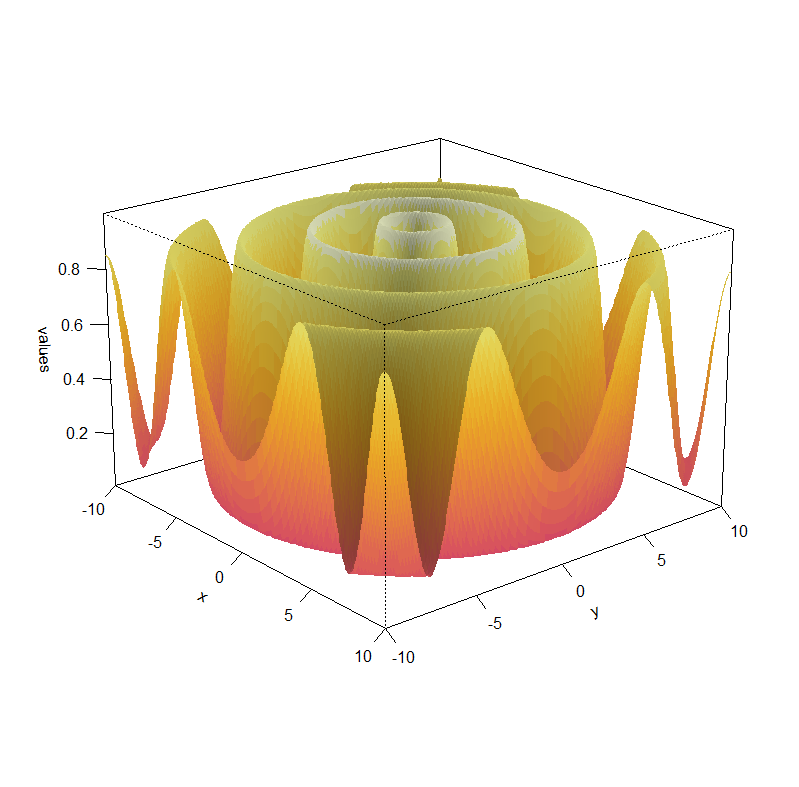
\includegraphics[scale=0.7]{img//roz03//Schaffer1_small_range.png}
%	\caption{Czas wykonania algorytmu HALS w zależności od rzędu faktoryzacji, liczba iteracji wew. 8}
%	\label{fig:HALStime}
%\end{figure}

\begin{equation} \label{eq:Schaffer1}
f(x)=0.5+\frac{\sin^2(x_1^2-x_2^2)-0.5}{[1+0.001(x_1^2+x_2^2)]^2}
\end{equation}


\begin{figure}
\centering
\begin{subfigure}{.5\textwidth}
  \centering
  \includegraphics[width=\linewidth]{{img//roz03//Schaffer1_full_range.png}}
  \caption{ Pełna dziedzina argumentów}
  \label{fig:sub1}
\end{subfigure}%
\begin{subfigure}{.5\textwidth}
  \centering
  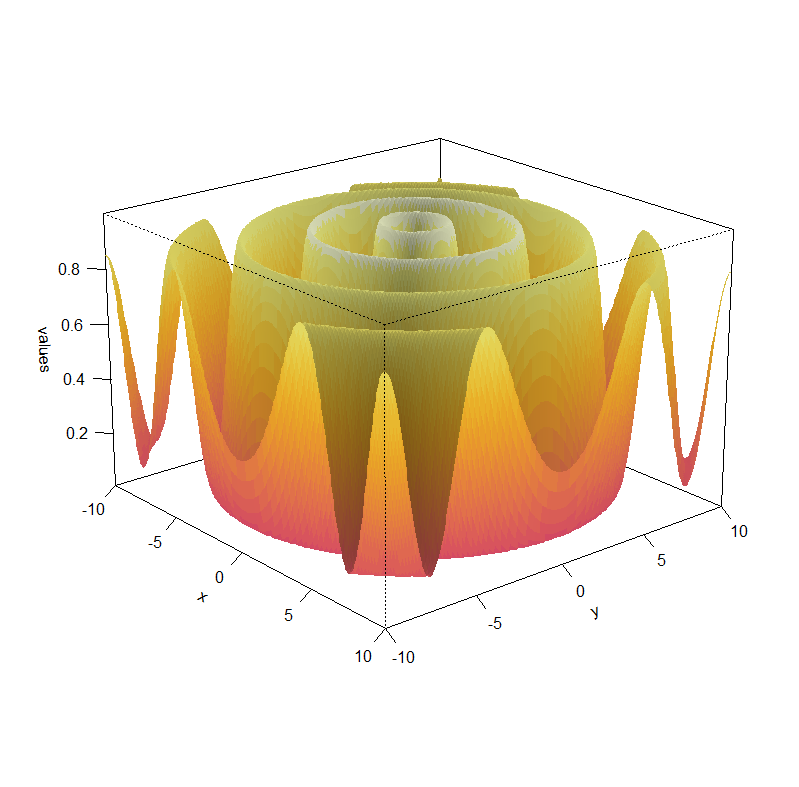
\includegraphics[width=\linewidth]{img//roz03//Schaffer1_small_range.png}
  \caption{Otoczenie ekstremum}
  \label{fig:sub2}
\end{subfigure}
\caption{Przebieg funkcji Schaffer1}
\label{fig:test}
\end{figure}


\subsection{Funkcja Paviani}
\begin{itemize}
\item wzor
\item dziedzina argumentow
\item optimum: jakie i gdzie
\item pewnie cos w necie ciekawego o nim jest
\end{itemize}
\begin{equation}\label{eq:Paviani}
f(x)=\sum_{i=1}^{10} \bigg(\log^2(x_i-2) + \log^2(10-x_i)\bigg) - \left(
\prod_{i=1}^{10} x_i\right)^{0.2}. 
\end{equation}
\section{Opis środowiska testowego}
\begin{itemize}
\item parametry maszyny testowej

\end{itemize}


\section{Przyjęte miary efektywności algorytmów}
\label{sec:przyjete_miary_efektywnosci_algorytmow}
wszstko dla tych samych liczby iteracji
\begin{enumerate}
\item najlepsze znalezione rozwiązanie kolejno w iteracjach
\item średnie rozwiązanie populacji kolejno w iteracjach
\item czas osiągnięcia rozwiązań 90, 95 i 99%

\end{enumerate}

\chapter{Rezultaty}
\section{Dobór parametrów algorytmu}
%\begin{itemize}
%\item tabelki z wyselekcjonowanymi parametrami, takie jak w excelu
%%\item wykres dla Schaffer1 bestfitness_calych_scenariuszy_Schaffer1 
%%\item fitness_etapow_scenariuszymutDefault_Schaffer1
%%\item fitness_etapow_scenariuszymutGauss_Schaffer1
%\end{itemize}
Przed przystąpieniem do badań porównujących efektywność badanych algorytmów konieczne jest określenie najlepszych konfiguracji ich parametrów. Dobór wartości parametrów algorytmów oparto na procedurze opisanej w podrozdziale \ref{sec:badane_scenariusze_doboru_parametrow}. Zdecydowano się na osobną selekcję parametrów dla każdej z wykorzystanych funkcji testowych, co w rezultacie pozwoliło na uzyskanie konfiguracji przedstawionych w tabelach \ref{table:selekcja_Schaffer_parametry}, \ref{table:selekcja_Paviani_parametry} i \ref{table:selekcja_Zeldasine_parametry}. Analizując tabele, pierwszym spostrzeżeniem (będącym potwierdzeniem intuicji) jest fakt uzyskiwania lepszych rezultatów przez algorytmy oparte na większych populacjach. Dlatego, w większości przypadków przyjęta konfiguracja składa się z maksymalnej rozpatrywanej liczby osobników. Zdominowanie parametru metody przeszukiwania lokalnego w algorytmach memetycznych przez metodę \emph{L-BFGS-B}, która jest domyślną wartością w implementacji pakietu \emph{GA} może być konsekwencją przyjętej miary porównawczej konfiguracji algorytmów. Już na poziomie dokumentacji pakietu pojawia się uwaga mówiąca, że \emph{L-BFGS-B} najczęściej uzyskuje najlepsze rezultaty, jednakże nie jest najszybszym z operatorów. Uwzględnienie czasu wykonania algorytmu jako współkryterium dla uzyskiwanego rozwiązania w procedurze selekcji parametrów algorytmów mogłoby w rezultacie przynieść potrzebę zmiany przyjmowaną metodę przeszukania lokalnego.

\begin{table}[ht]
\caption{Dobrane wartości parametrów algorytmów dla funkcji \emph{Schaffer nr 2}}
\label{table:selekcja_Schaffer_parametry}
\begin{center}
\begin{tabular}{|c|c|c|c|c|c|c|c|}
	\hline
	Algorytm & Mutacja & $p_{mut}$ & $p_{cross}$ & $r_{pop}$ & $p_{opt}$ & $p_{sel}$ & Operator\\
	\hline
	Memetyczny & \emph{mutDefault} & 0.5 & 0.9 & 100 & 0.8 & 1.0 & \emph{L-BFGS-B} \\
	Memetyczny & \emph{mutGauss}  & 0.7 & 0.9 & 100 & 1.0 & 0.6 & \emph{L-BFGS-B} \\
	Genetyczny & \emph{mutDefault} & 0.6 & 0.9 & 100 & - & - & - \\
	Genetyczny & \emph{mutGauss}  & 0.5 & 1.0 & 100 & - & - & - \\
	\hline
	\end{tabular}

\begin{tabular}{|c|c|c|c|c|}
	\hline
	Algorytm & $\phi_1$ & $\phi_2$ & $w$ & $r_{pop}$ \\
	\hline
	PSO & 1.6 & 2.5 & 1.0 & 100 \\
	\hline
\end{tabular}
\end{center}
\end{table}
  
\begin{table}[ht]
\caption{Dobrane wartości parametrów algorytmów dla funkcji \emph{Paviani}}
\label{table:selekcja_Paviani_parametry}
\begin{center}
\begin{tabular}{|c|c|c|c|c|c|c|c|}
	\hline
	Algorytm & Mutacja & $p_{mut}$ & $p_{cross}$ & $r_{pop}$ & $p_{opt}$ & $p_{sel}$ & Operator\\
	\hline
	Memetyczny & \emph{mutDefault} & 0.5 & 0.7 & 100 & 1.0 & 1.0 & \emph{L-BFGS-B} \\
	Memetyczny & \emph{mutGauss}  & 0.8 & 0.9 & 100 & 1.0 & 0.9 & \emph{L-BFGS-B} \\
	Genetyczny & \emph{mutDefault} & 0.8 & 0.7 & 100 & - & - & - \\
	Genetyczny & \emph{mutGauss}  & 1.0 & 1.0 & 100 & - & - & - \\
	\hline
	\end{tabular}

\begin{tabular}{|c|c|c|c|c|}
	\hline
	Algorytm & $\phi_1$ & $\phi_2$ & $w$ & $r_{pop}$ \\
	\hline
	PSO & 1.0 & 3.1 & 0.8 & 100 \\
	\hline
\end{tabular}
\end{center}
\end{table}

\begin{table}[ht]
\caption{Dobrane wartości parametrów algorytmów dla funkcji \emph{ZeldaSine10}}
\label{table:selekcja_Zeldasine_parametry}
\begin{center}
\begin{tabular}{|c|c|c|c|c|c|c|c|}
	\hline
	Algorytm & Mutacja & $p_{mut}$ & $p_{cross}$ & $r_{pop}$ & $p_{opt}$ & $p_{sel}$ & Operator\\
	\hline
	Memetyczny & \emph{mutDefault} & 0.7 & 1.0 & 100 & 0.6 & 0.6 & \emph{L-BFGS-B} \\
	Memetyczny & \emph{mutGauss}  & 0.9 & 1.0 & 50 & 1.0 & 0.6 & \emph{L-BFGS-B} \\
	Genetyczny & \emph{mutDefault} & 0.8 & 0.9 & 100 & - & - & - \\
	Genetyczny & \emph{mutGauss}  & 0.9 & 1 & 100 & - & - & - \\
	\hline
	\end{tabular}

\begin{tabular}{|c|c|c|c|c|}
	\hline
	Algorytm & $\phi_1$ & $\phi_2$ & $w$ & $r_{pop}$ \\
	\hline
	PSO & 1.6 & 2.5 & 1.0 & 100 \\
	\hline
\end{tabular}
\end{center}
\end{table}

\par
W tabelach \ref{table:selekcja_Schaffer_czasy}, \ref{table:selekcja_Paviani_czasy} i \ref{table:selekcja_Zeldasine_czasy} zaprezentowano uśrednione najlepsze rozwiązania znajdowane przy wykorzystaniu wyselekcjonowanych konfiguracji algorytmów w ramach selekcji, tj. przy wykorzystaniu zaledwie 5 pierwszych pokoleń. W przypadku algorytmów memetycznych przedstawiono również, który z omówionych w podrozdziale \ref{sec:badane_scenariusze_doboru_parametrow} scenariuszy ostatecznie uzyskał najlepsze rezultaty. W  tym miejscu można zauważyć zależność pomiędzy trudnością funkcji testowych i kompletnością zwycięskiego scenariusza. Dokładna analiza wykonania algorytmu memetycznego dla funkcji \emph{Zeldasine10} wykazała, że wykorzystany operator \emph{L-BFGS-B} bardzo szybko znajduje optymalne rozwiązanie. W takiej sytuacji, gdzie wiele scenariuszy pozwala na osiąganie optimum funkcji kluczowym parametrem wyboru scenariusza staje się czas jego wykonania. 

\begin{table}[ht]
\caption{Czasy i najlepsze rozwiązanie znalezione w trakcie selekcji parametrów algorytmów dla funkcji \emph{Schaffer nr 2}}
\label{table:selekcja_Schaffer_czasy}
\begin{center}
\begin{tabular}{|c|c|c|c|c|}
	\hline
	Algorytm & Mutacja & Najlepsze rozwiązanie & Czas selekcji [s] & Scenariusz \\
	\hline
	Memetyczny & \emph{mutDefault} & 0.03788 & 540.74 & $[1-2-3,\; 4-5-6]$\\
	Memetyczny & \emph{mutGauss} & 0.02769 & 584.67 & $[1-2-3,\; 4-5-6]$ \\
	Genetyczny & \emph{mutDefault} & 0.06609 & 171.79 & - \\
	Genetyczny & \emph{mutGauss} & 0.04549 & 186.90 & - \\
	PSO	& - & 0.09882 & 282.22 & -\\

	\hline
	\end{tabular}
\end{center}
\end{table}            

\begin{table}[ht]
\caption{Czasy i najlepsze rozwiązanie znalezione w trakcie selekcji parametrów algorytmów dla funkcji \emph{Paviani}}
\label{table:selekcja_Paviani_czasy}
\begin{center}
\begin{tabular}{|c|c|c|c|c|}
	\hline
	Algorytm & Mutacja & Najlepsze rozwiązanie & Czas selekcji [s] & Scenariusz \\
	\hline
	Memetyczny & \emph{mutDefault} & -45.77847 & 849.00 & $[4-5-6,\; 1-2-3]$\\
	Memetyczny & \emph{mutGauss} & -45.77847 & 841.99 & $[4-5-6,\; 1-2-3]$ \\
	Genetyczny & \emph{mutDefault} & -24.71857 & 212.64 & - \\
	Genetyczny & \emph{mutGauss} & -23.36381 & 218.80 & - \\
	PSO	& - & -37.78442 & 412.75 & -\\

	\hline
	\end{tabular}
\end{center}
\end{table}




\begin{table}[ht]
\caption{Czasy i najlepsze rozwiązanie znalezione w trakcie selekcji parametrów algorytmów dla funkcji \emph{ZeldaSine10}}
\label{table:selekcja_Zeldasine_czasy}
\begin{center}
\begin{tabular}{|c|c|c|c|c|}
	\hline
	Algorytm & Mutacja & Najlepsze rozwiązanie & Czas selekcji [s] & Scenariusz \\
	\hline
	Memetyczny & \emph{mutDefault} & -3.5 & 243.22 & $[4-5,\;3-6,\;1-2]$\\
	Memetyczny & \emph{mutGauss} & -3.5 & 190.31 & $[4-5,\;3-6,\;1-2]$ \\
	Genetyczny & \emph{mutDefault} & -1.69261 & 206.83 & - \\
	Genetyczny & \emph{mutGauss} & -1.81252 & 214.95 & - \\
	PSO	& - & -0.91760 & 36.15 & -\\

	\hline
	\end{tabular}
\end{center}
\end{table}

Jednym z celów realizowanej pracy było sprawdzenie skuteczności zaproponowanych w rozdziale \ref{ch:przyjety_model_doboru_parametrow_algorytmu} scenariuszy doboru kolejnych wartości parametrów algorytmów memetycznych w celu ograniczenia liczby sprawdzanych kombinacji bez znaczącej straty jakości przyjętej konfiguracji. Z powodu ograniczeń technicznych nie zdecydowano się na porównawcze wykonanie pełnego przeglądu wszystkich możliwych kombinacji, więc scenariusze porównane zostaną jedynie między sobą pod kątem uzyskanych rezultatów i czasu wykonania. Na wykresach \ref{fig:parameter_selection_fitness_overall}, \ref{fig:parameter_selection_fitness_in_phases}, \ref{fig:parameter_selection_time_overall} i \ref{fig:parameter_selection_time_in_phases} przedstawione zostało porównanie dla funkcji \emph{Schaffer nr 2}. Analogiczne wykresy dla pozostałych przyjętych funkcji testowych zamieszczono w dodatku \ref{ch:dodatekC-wykresy}.

\par
Jak przedstawiono na wykresie \ref{fig:parameter_selection_fitness_overall}, konfiguracja uzyskana poprzez zastosowanie scenariusza $[1-2-3,\,4-5-6]$ pozwala na uzyskanie najlepszych rezulatów, jednakże scenariusz $[3-6,\,1-2,\,4-5]$ jest tylko nieznacznie gorszy. Dodatkowo, porównując wspomniane dwa scenariusze na podstawie wykresu \ref{fig:parameter_selection_time_overall} można stwierdzić, że uzyskanie nieznacznie lepszego rozwiązania wymagało aż trzykrotnie dłuższych obliczeń. Zestawiając ze sobą te dwa wyróżniające się pod kątem jakości uzyskanej konfiguracji scenariusze można stwierdzić, że oba z nich są równie użyteczne, ale w odniesieniu do różnych potrzeb wykorzystania. Jeśli priorytetem będzie maksymalna możliwa jakość parametrów algorytmów to lepszym będzie scenariusz $[1-2-3,\,4-5-6]$, natomiast jeśli ważniejszy będzie czas selekcji parametrów, to $[3-6,\,1-2,\,4-5]$. Zdecydowanie się na szybszy scenariusz może pozwolić na zwiększenie zbiorów sprawdzanych wartości parametrów, a przez to zwiększenie jakości uzyskanej konfiguracji algorytmu. Należy jednak po raz kolejny zaznaczyć, że skuteczność scenariuszy bezpośrednio zależy od trudności optymalizowanej funkcji.
\par
Analizując wykres \ref{fig:parameter_selection_fitness_in_phases} przedstawiający rezultaty uzyskane w kolejnych etapach selekcji można zauważyć niespodziewane wyniki dla scenariusza $[4-5,\,3-6,\,1-2]$ z operatorem \emph{mutDefault} oraz $[1-2-3,\,4-5-6]$ z \emph{mutGauss} wskazujące na to, że przeprowadzony kolejny etap selekcji pogorszył otrzymywane rozwiązanie. Może to wskazywać na sytuację, w której przy danej kombinacji pozostałych parametrów tymczasowo przyjęte domyślne wartości parametrów pozwalają na uzyskanie lepszych rezultatów niż którakolwiek z testowanych kombinacji danego etapu selekcji. Gdyby taka sytuacja była obserwowana w większej liczbie scenariuszy lub rozwiązanie w kolejnych etapach pogarszałoby się w znaczący sposób, należałoby zmienić zakres testowanych wartości parametrów w stronę domyślnych zaimplementowanych w pakiecie \emph{GA}.
\par
W sytuacji, gdy jakość konfiguracji uzyskana najlepszym pod tym kątem scenariuszem nie jest wystarczająca, można posłużyć się danymi czasu wykonania kolejnych etapów selekcji przedstawionymi na wykresie \ref{fig:parameter_selection_time_in_phases}. Przedstawia on czas wykonania kolejnych etapów selekcji. Na tej podstawie można zdecydować, któremu z parametrów można rozszerzyć zbiór sprawdzanych wartości bez diametralnego wydłużenia czasu wykonania całego scenariusza. Z drugiej strony, jeśli celem jest skrócenie czasu wykonania scenariusza na podstawie wykresu można określić, zbiory których parametrów należy ograniczyć.
\begin{figure}[h] 
\centering
  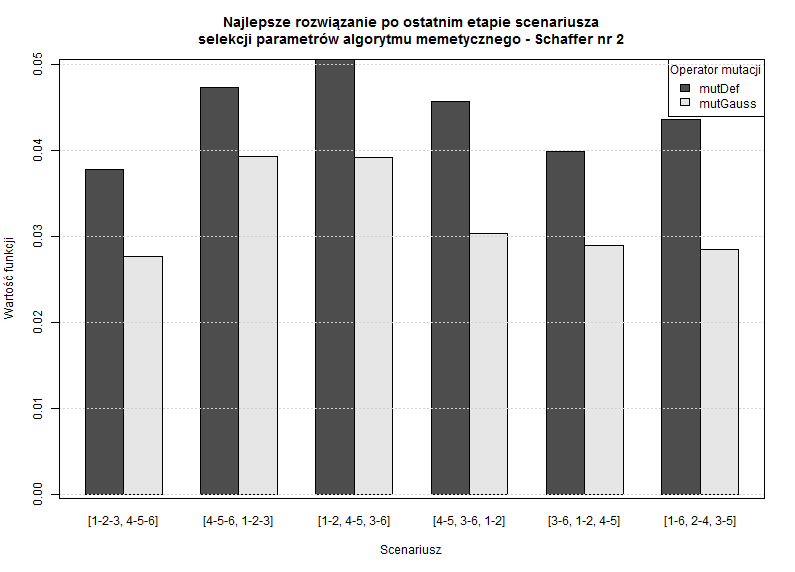
\includegraphics[width=\linewidth]{{img//roz04//parameterSelection//bestfitness_calych_scenariuszy_Schaffer1.png}}
\caption{Porównanie najlepszego rozwiązania dla różnych scenariuszy dla funkcji \emph{Schaffer nr 2}}
\label{fig:parameter_selection_fitness_overall}
\end{figure}


\begin{figure}[ht] 
\centering
\begin{subfigure}{\textwidth}
  \centering
  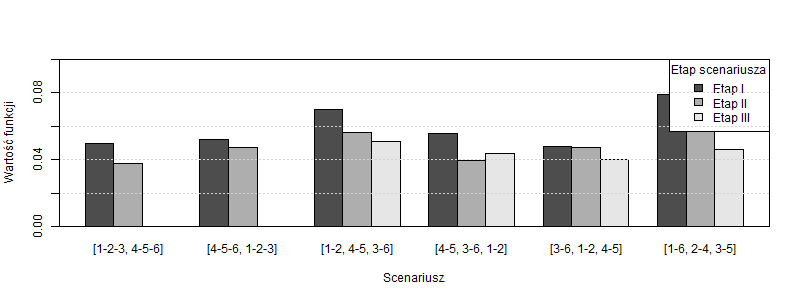
\includegraphics[width=\linewidth]{{img//roz04//parameterSelection//fitness_etapow_scenariuszymutDefault_Schaffer1.png}}
  \caption{\emph{mutDefault}}
  %\label{fig:sub1}
\end{subfigure}
\begin{subfigure}{\textwidth}
  \centering
  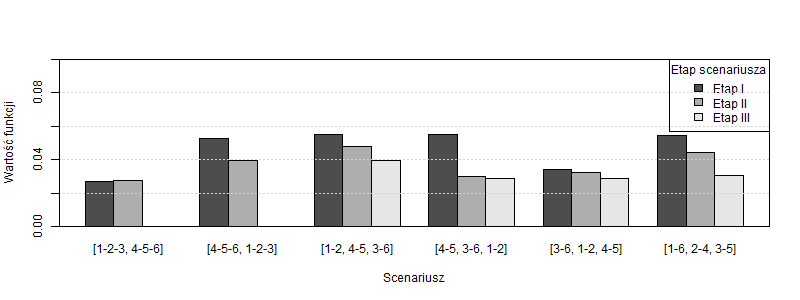
\includegraphics[width=\linewidth]{img//roz04//parameterSelection//fitness_etapow_scenariuszymutGauss_Schaffer1.png}
  \caption{\emph{mutGauss}}
  %\label{fig:sub2}
\end{subfigure}
\caption{Najlepsze znajdywane rozwiązanie kolejno w etapach selekcji dla funkcji \emph{Schaffer nr 2}}
\label{fig:parameter_selection_fitness_in_phases}
\end{figure}

\begin{figure}[h] 
\centering
  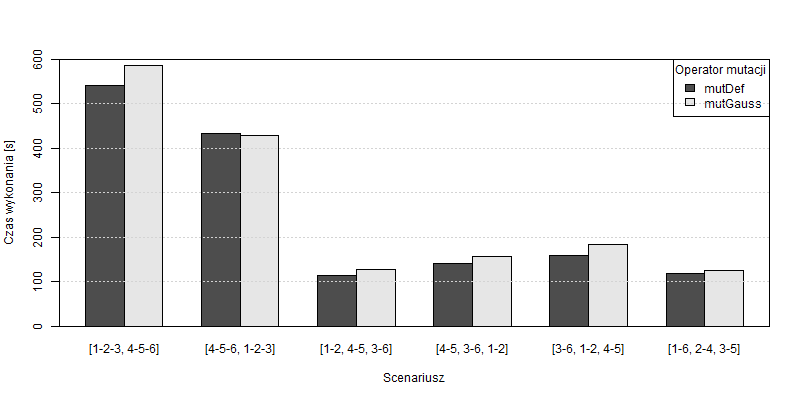
\includegraphics[width=\linewidth]{{img//roz04//parameterSelection//czas_calych_scenariuszy_Schaffer1.png}}
\caption{Czas wykonania różnych scenariuszy dla funkcji \emph{Schaffer nr 2}}
\label{fig:parameter_selection_time_overall}
\end{figure}


\begin{figure}[ht] 
\centering
\begin{subfigure}{\textwidth}
  \centering
  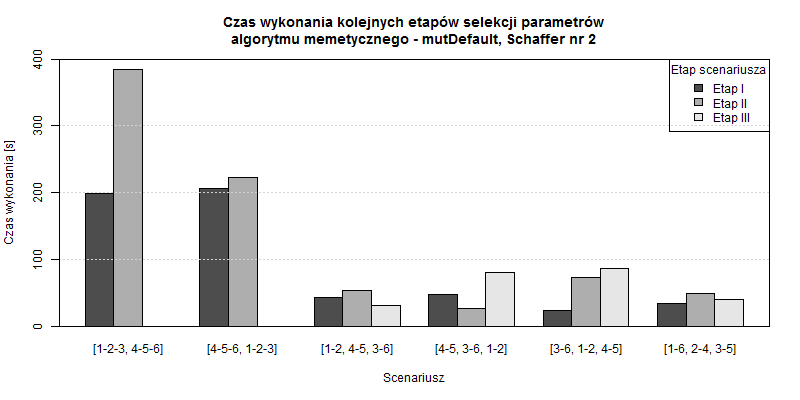
\includegraphics[width=\linewidth]{{img//roz04//parameterSelection//czas_etapow_scenariuszymutDefault_Schaffer1.png}}
  \caption{\emph{mutDefault}}
\end{subfigure}
\begin{subfigure}{\textwidth}
  \centering
  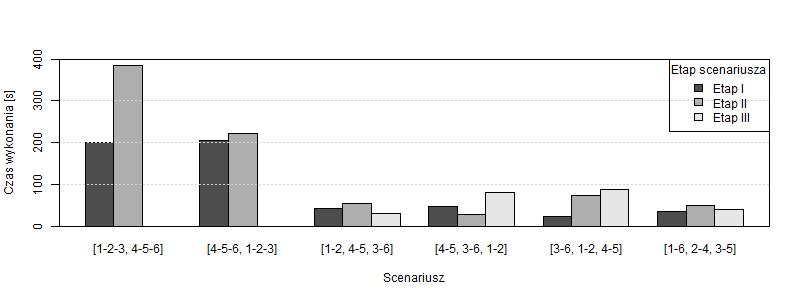
\includegraphics[width=\linewidth]{img//roz04//parameterSelection//czas_etapow_scenariuszymutGauss_Schaffer1.png}
  \caption{\emph{mutGauss}}
\end{subfigure}
\caption{Czas wykonania kolejnych etapów selekcji dla funkcji \emph{Schaffer nr 2}}
\label{fig:parameter_selection_time_in_phases}
\end{figure}

\FloatBarrier

\section{Wyniki względem miar efektywności}
\subsection{Kryterium nr 1 - najlepsze rozwiązanie}

%\begin{itemize}
%\item we wszystich przypadkach PSO wyszło najgorzej
%\item dla Schaffera mutGauss cał zauwazalnie lepsze rezultaty, bo pozniej osiągał zbieżność
%\item tam, gdzie nie było problemem znalezienie optymalnego rozwiazania mutGauss osiągał zbieżność wcześniej, a więc szybciej znajdował rozwiązanie
%\end{itemize}
\par
Badania porównawcze według tego kryterium opierały się na określeniu średniego najlepszego rozwiązania znajdowanego do osiągnięcia zbieżności populacji. Za oznakę zbieżności przyjęto brak polepszenia rezultatu przez 50 iteracji algorytmu. Oprócz porównania ze sobą rożnych algorytmów wykresy uwidaczniają różnicę pomiędzy wykorzystanymi operatorami mutacji. 
\par
W przypadku każdej z użytych funkcji testowych algorytm \emph{PSO} osiąga zbieżność w nieznacznie większej liczbie iteracji niż algorytm memetyczny, jednakże rozwiązania przez niego uzyskiwane są znacznie gorsze niż dla pozostałych metod optymalizacji. 
\par 
Zgodnie z tym, co zauważono już na etapie doboru parametrów algorytmów  najtrudniejszą, z punktu widzenia znalezienia optimum, funkcją okazała się \emph{Schaffer nr 2}. Wykres \ref{fig:kryt1_Schaffer} można rozumieć w taki sposób, że algorytm genetyczny i memetyczny z operatorem \emph{mutDefault} osiągają bardzo zbliżone rezultaty, jednakże memetyczny osiąga zbieżność w znacznie mniejszej liczbie iteracji. Operator \emph{mutGauss} pozwolił na uzyskanie lepszych rozwiązań niż \emph{mutDefault}, choć rożnie wpłynął na szybkość uzyskania zbieżności - w memetycznym zwiększył liczbę potrzebnych iteracji, a w genetycznym zmniejszył. 

\begin{figure}[ht]
\begin{subfigure}{.5\textwidth}
  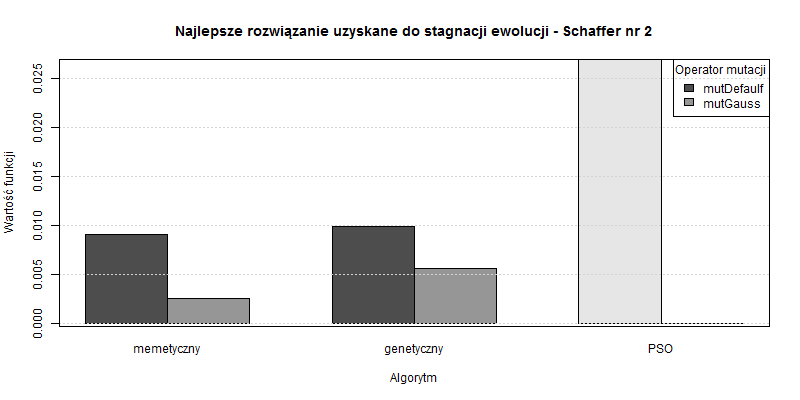
\includegraphics[width=\linewidth]{{img//roz04//kryt1//kryt1_bestFitness_Schaffer.png}}
  \caption{Rozwiązanie}
  \label{fig:kryt1_Schaffer_fitness}
\end{subfigure}%
\begin{subfigure}{.5\textwidth}
  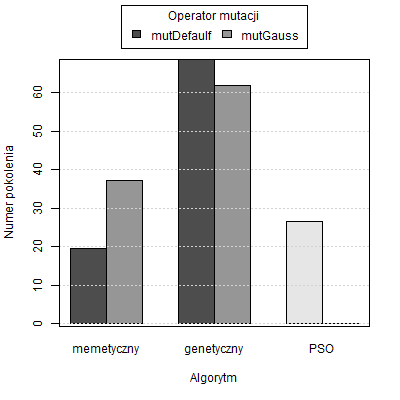
\includegraphics[width=\linewidth]{img//roz04//kryt1//kryt1_nr_generacji_stagnacji_Schaffer.png}
  \caption{Numer pokolenia}
  \label{fig:kryt1_Schaffer_stagnation}
\end{subfigure}
\caption{Określenie momentu stagnacji optymalizacji - \emph{Schaffer nr 2}}
\label{fig:kryt1_Schaffer}
\end{figure}

%%%%%%%%%%%%%%%%%%%%%%%%%%%%%%%%%%%%%%%%%%

\par
W przypadku funkcji \emph{Paviani}, tylko algorytm memetyczny zdołał osiągnąć rozwiązanie optymalne. Algorytm genetyczny uzyskiwał rezultaty bardzo bliskie optimum i ich dokładne wartości przedstawiono w tabeli \ref{table:kryt1_Paviani_best_fitness}. Podobnie jak w przypadku \emph{Schaffer nr 2}, operator \emph{mutDefault} opóźnił zbieżność algorytmu memetycznego, a przyspieszył genetycznego. Ponownie mutacja gaussowska pozwoliła na znalezienie lepszego rozwiązania niż domyślna w pakiecie \emph{GA}. Porównanie algorytmów według tego kryterium  dla \emph{Paviani} przedstawiono na wykresie \ref{fig:kryt1_Paviani}.


\begin{table}[hbt]
\caption{Rozwiązania dla funkcji Paviani}
\label{table:kryt1_Paviani_best_fitness}
\begin{center}
\begin{tabular}{|c|c|c|}
	\hline
	\multirow{2}{*}{Algorytm}& \multicolumn{2}{c|}{Operator mutacji} \\
	\cline{2-3}
	{} & \emph{mutDefault} & \emph{mutGauss} \\
	\hline
	\emph{Memetyczny} & -45.77847 & -45.77847\\
	\emph{Genetyczny} & -45.53228 & -45.77498\\
	\hline
	\emph{PSO} & \multicolumn{2}{c|}{-40.45703}\\
	\hline
	\end{tabular}
\end{center}
\end{table}

\begin{figure}[ht]
\begin{subfigure}{.5\textwidth}
  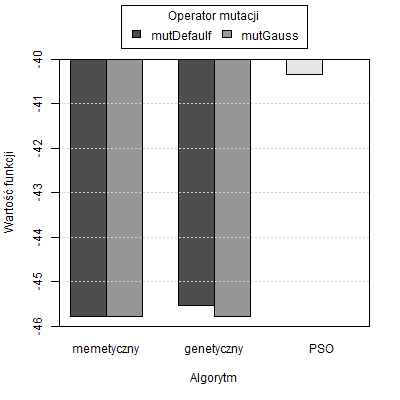
\includegraphics[width=\linewidth]{{img//roz04//kryt1//kryt1_bestFitness_Paviani.png}}
  \caption{Rozwiązanie}
  \label{fig:kryt1_Paviani_fitness}
\end{subfigure}%
\begin{subfigure}{.5\textwidth}
  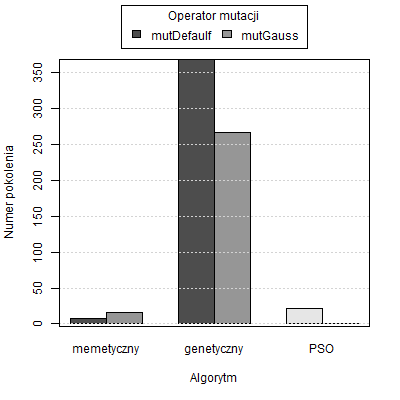
\includegraphics[width=\linewidth]{img//roz04//kryt1//kryt1_nr_generacji_stagnacji_Paviani.png}
  \caption{Numer pokolenia}
  \label{fig:kryt1_Paviani_stagnation}
\end{subfigure}
\caption{Określenie momentu stagnacji optymalizacji - \emph{Paviani}}
\label{fig:kryt1_Paviani}
\end{figure}

%%%%%%%%%%%%%%%%%%%%%%%%%%%%%%%%%%%%%%%%%%
\par
Dla funkcji \emph{ZeldaSine10}, w przeciwieństwie do pozostałych, algorytm memetyczny z operatorem \emph{mutGauss} uzyskał gorsze rozwiązania od wersji z \emph{mutDefault}, ale i również od obu wariantów genetycznego. Podobnie jak dla \emph{Schaffer nr 2} i \emph{Paviani}, \emph{mutGauss} opóźnił stagnację optymalizacji algorytmem memetycznym, i przyspieszył w genetycznym. Na wykresie \ref{fig:kryt1_Zeldasine} przedstawiono rezultaty wskazujące na około piętnastokrotną różnicę w szybkości osiągania stagnacji optymalizacji pomiędzy memetyczną i genetyczną metoda rozwiązywania problemów optymalizacyjnych. 

\begin{figure}[ht] 
\begin{subfigure}{.5\textwidth}
  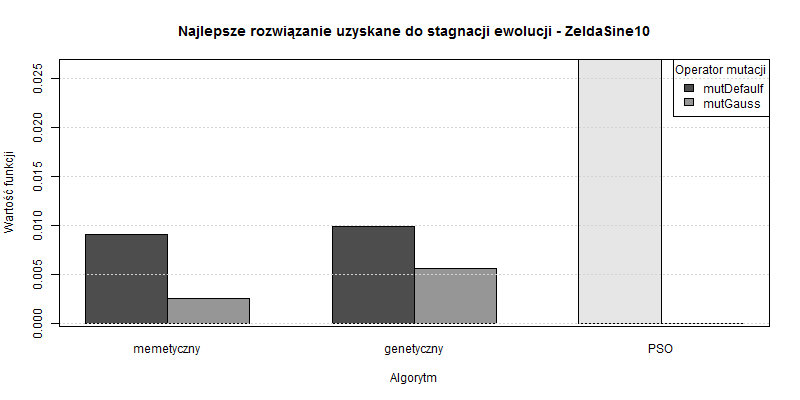
\includegraphics[width=\linewidth]{{img//roz04//kryt1//kryt1_bestFitness_Zeldasine.png}}
  \caption{Rozwiązanie}
  \label{fig:kryt1_Zeldasine_fitness}
\end{subfigure}%
\begin{subfigure}{.5\textwidth}
  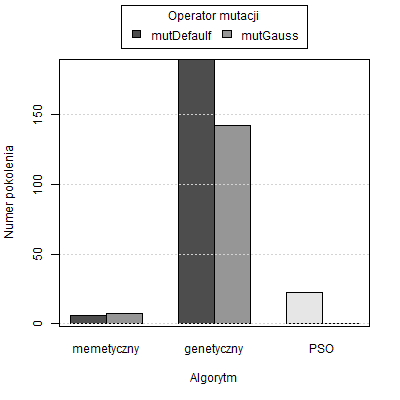
\includegraphics[width=\linewidth]{img//roz04//kryt1//kryt1_nr_generacji_stagnacji_Zeldasine.png}
  \caption{Numer pokolenia}
  \label{fig:kryt1_Zeldasine_stagnation}
\end{subfigure} 
\caption{Określenie momentu stagnacji optymalizacji - \emph{ZeldaSine10}}
\label{fig:kryt1_Zeldasine}
\end{figure}

\FloatBarrier

\par
Końcowym wnioskiem podsumowującym porównanie algorytmów według \emph{kryterium nr 1} jest niepodważalna przewaga algorytmu memetycznego jeśli chodzi o liczbę koniecznych iteracji do uzyskania rozwiązania optymalnego lub mu bliskiego. W większości przypadków operator \emph{mutGauss} okazuje się uzyskiwać lepsze rezultaty niż \emph{mutDefault}, jednakże różnie wpływa na szybkość stagnacji procesu optymalizacji. Algorytm \emph{PSO} kończył optymalizację w nieznacznie większej liczbie iteracji niż memetyczny, jednakże uzyskiwał najgorsze rozwiązania.


\subsection{Kryterium nr 2 - szybkość osiągania rozwiązania}
%
%\begin{itemize}
%\item z uwagi na dużo dłuższe czasy dla PSO i progu 99\% zamieszczono dwa wykresy dla każdej funkcji
%\item nieosiągnięcie przez algorytm danego progu w ciągu 30 sekund prezentowane jest jako wartość -0.1
%\item nietypowym rezultatem jest nieosiągnięcie przez algorytm memetyczny-mutDefault dla Schaffera progu 99\%
%\item najlepsze rezultaty uzyskano algorytmem memetycznym, a w szczególności z wykorzystaniem mutGauss
%\item ewidentnie PSO ma problem z optymalizacją Zeldasine, nawet nie uzyskał progu 50\%
%\end{itemize}

\par
\emph{Kryterium nr 2} pozwala porównać szybkość osiągania określonych rezultatów w zależności od czasu wykonania algorytmu, a nie liczby potrzebnych iteracji. W tabeli \ref{table:kryt2_wartosci_progow} przedstawiono jakie wartości funkcji dopasowania odpowiadają kolejnym przyjętym progom jakości otrzymanego rozwiązania. Bardzo wąski ogólny zakres wartości funkcji \emph{Schaffer nr 2} wpłynął na stopień trudności osiągnięcia najwyższych zdefiniowanych progów. Granicznym czasem wykonania algorytmu jest \emph{30 sekund}. Przypadek nieosiągnięcia danego progu w żadnej z 30 prób pomiarowych oznaczany jest na wykresach \ref{fig:kryt2_Schaffer}, \ref{fig:kryt2_Paviani} i \ref{fig:kryt2_Zeldasine} wartością $-0.1$. Wszystkie pomiary zostały przeprowadzone po przyjęciu dokładności pomiaru równej $50 ms$. Czasy uzyskane przez algorytm \emph{PSO} oraz progu $99\%$ okazały się znacznie dłuższe niż w pozostałych przypadkach, więc zdecydowano się na przedstawienie rezultatów na dwóch wykresach dla każdej z funkcji - pierwszy z nich opisuje wszystkie rezultaty dla funkcji testowej, a drugi nie zawiera \emph{PSO} i progu $99\%$.
\par
Podobnie jak w przypadku \emph{kryterium nr 1} algorytm \emph{PSO} okazał się najgorszym z badanych metod optymalizacji dla wszystkich trzech funkcji testowych. Osiągał kolejne progi w około pięciokrotnie dłuższym czasie lub nie osiągał ich w założonym maksymalnym okresie. 


\begin{table}[ht]
\caption{Wartości kolejnych progów dokładności rozwiązania}
\label{table:kryt2_wartosci_progow}
\begin{center}
\begin{tabular}{|c|c|c|c|c|c|}
	\hline
	\multirow{2}{*}{Funkcja}& \multicolumn{5}{c|}{Próg} \\
	\cline{2-6}
	{} & 50\% & 75\% & 90\% & 95\% & 99\% \\
	\hline
	\emph{Schaffer nr 2} & 0.25227 & 0.12614 & 0.05045 & 0.02523 & 0.00504\\
	\emph{Paviani} & -22.42884 & -34.10365 & -41.10854 & -43.44351 & -45.31148\\
	\emph{ZeldaSine10} & -1.92663 & -2.71331 & -3.18532 & -3.34266 & -3.46853\\
	\hline
	\end{tabular}
\end{center}
\end{table}

\par
W przypadku funkcji \emph{Schaffer nr 2}, dla której rezultaty przedstawiono na wykresie \ref{fig:kryt2_Schaffer}, najlepszą z testowanych metod okazał się algorytm memetyczny z wykorzystaniem mutacji gaussowskiej. Uzyskał on najniższy czas osiągnięcia progu $99\%$, mimo iż próg $95\%$ szybciej uzyskano algorytmem genetycznym, co widać na wykresie \ref{fig:kryt2_Schaffer_restricted}. Żadna z badanych metod nie miał trudności z osiągnięciem progu $95\%$. Ciekawie wygląda zestawienie wyników dla dwóch najwyższych progów. Dla algorytmu memetycznego operator \emph{mutGauss} dla obu poziomów dokładności uzyskiwał lepsze rezultaty niż \emph{mutDefault}, zaś dla algorytmu genetycznego w przypadku progu $99\%$ domyślny operator osiągał rozwiązanie z krótszym czasie. Dla progu $95\%$ nieznaczną przewagę czasową posiadał algorytm genetyczny, jednakże dla ostatniego progu uzyskał znacznie gorsze rezultaty  rezultaty niż memetyczny z \emph{mutGauss}. Niespodziewanie, algorytm memetyczny z \emph{mutDefault} nie osiągnął progu $99\%$ w żadnej z prób testowych. 


%%%%%%%%%%%%%%%%%%%%%%%%%%%%%%%%%%%%%%%%%
\begin{figure}[ht] 
\centering
\begin{subfigure}{\textwidth}
  \centering
  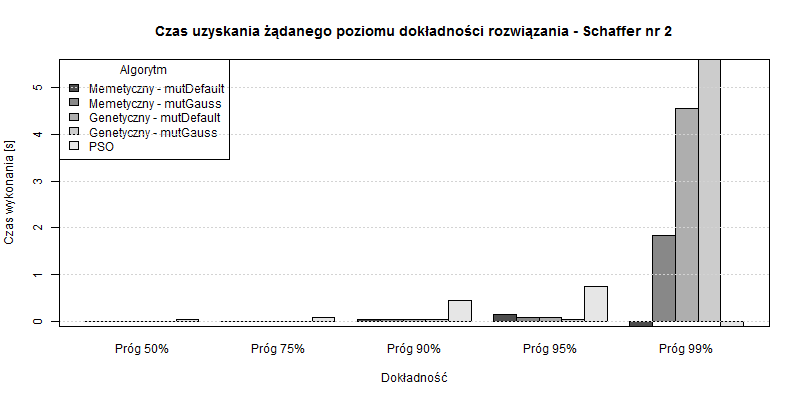
\includegraphics[width=\linewidth]{{img//roz04//kryt2//kryt2_czas_uzyskania_poziomu_dokladnosci_Schaffer.png}}
  \caption{Wszystkie algorytmy i progi dokładności}
\end{subfigure} 
\begin{subfigure}{\textwidth}
  \centering
  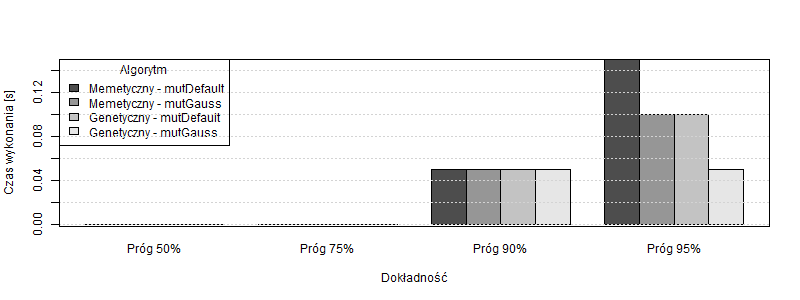
\includegraphics[width=\linewidth]{img//roz04//kryt2//kryt2_czas_uzyskania_poziomu_dokladnosci_bez_PSO_Schaffer.png}
  \caption{Wszystkie algorytmy i progi dokładności z wyłączeniem PSO i progu 99\%}
 \label{fig:kryt2_Schaffer_restricted}
\end{subfigure} 
\caption{Czas osiągnięcia rozwiązania o zadanej dokładności - \emph{Schaffer nr 2}}
\label{fig:kryt2_Schaffer}
\end{figure}
%%%%%%%%%%%%%%%%%%%%%%%%%%%%%%%%%%%%%%%%%%%%
\FloatBarrier
\par
Badania dla tego kryterium z wykorzystaniem funkcji \emph{Paviani} jednoznacznie wskazują na przewagę algorytmu memetycznego nad pozostałymi. Wyniki przedstawiono na wykresie \ref{fig:kryt2_Paviani}. Niezależnie od wykorzystanego operatora mutacji, osiągnął on kolejne progi w najniższym możliwym czasie. Może to być efektem tego, że wykorzystana metoda \emph{L-BFGS-B} bardzo dobrze radzi sobie z funkcjami podobnymi do \emph{Paviani}. W przypadku algorytmu genetycznego możliwe jest już porównanie operatorów ze sobą - dla wszystkich progów poza $99\%$ \emph{mutDefault} uzyskiwał niższe czasy niż  mutacja gaussowska. Dla ostatniego progu relacja uległa odwróceniu - czas potrzebny algorytmowi genetycznemu opartemu o \emph{mutGauss} jest dwukrotnie niższy niż dla \emph{mutDefault}. Co więcej, różnica w czasie pomiędzy progiem $95\%$ i $99\%$ dla \emph{mutGauss} wynosi około $25\%$ , a dla \emph{mutDefualt} około $150\%$. 

%%%%%%%%%%%%%%%%%%%%%%%%%%%%%%%%%%%%%%%%%%
\begin{figure}[ht] 
\centering
\begin{subfigure}{\textwidth}
  \centering
  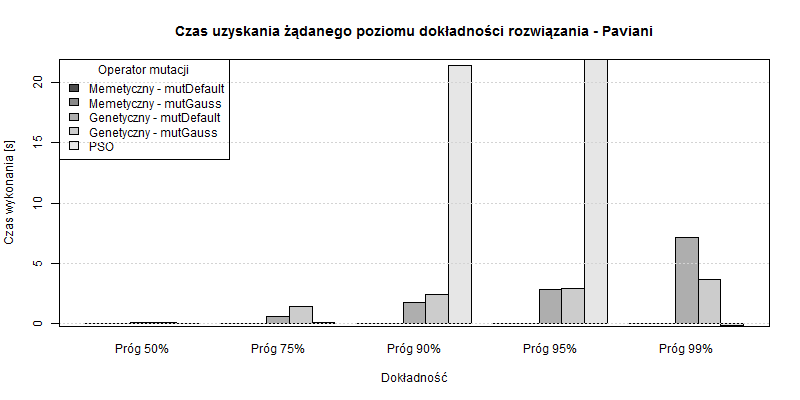
\includegraphics[width=\linewidth]{{img//roz04//kryt2//kryt2_czas_uzyskania_poziomu_dokladnosci_Paviani.png}}
  \caption{Wszystkie algorytmy i progi dokładności}
\end{subfigure}
\begin{subfigure}{\textwidth}
  \centering
  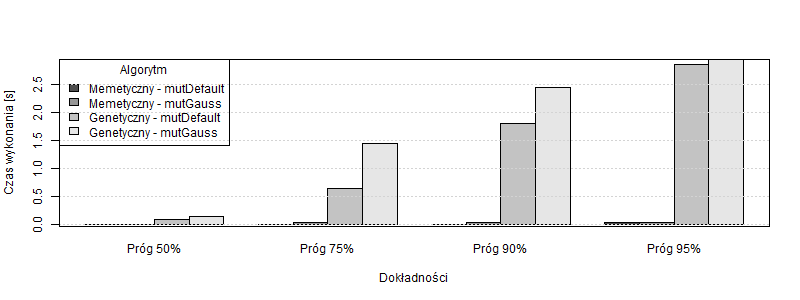
\includegraphics[width=\linewidth]{img//roz04//kryt2//kryt2_czas_uzyskania_poziomu_dokladnosci_bez_PSO_Paviani.png}
  \caption{Wszystkie algorytmy i progi dokładności z wyłączeniem PSO i progu 99\%}
\end{subfigure}
\caption{Czas osiągnięcia rozwiązania o zadanej dokładności - \emph{Paviani}}
\label{fig:kryt2_Paviani}
\end{figure}
%%%%%%%%%%%%%%%%%%%%%%%%%%%%%%%%%%%%%%%%%%%
\FloatBarrier
\par
W przypadku ostatniej z wykorzystanej funkcji testowych otrzymane rezultaty wydają się sprzeczne z intuicją. Na wykresie \ref{fig:kryt2_Zeldasine} przedstawiono wyniki wskazujące na to, że ostatnie dwa progi dokładności rozwiązania nie są osiągane przez algorytm memetyczny z \emph{mutDefault}, pomimo , że algorytm genetyczny z tym samym operatorem mutacji osiąga je w czasie $2.15$ sekundy. Porównując skuteczność mechanizmów mutacji ze sobą ponownie można zauważyć przewagę \emph{mutGauss} nad \emph{mutDefault}. Funkcja \emph{ZeldaSine10} sprawia duże problemy algorytmowi \emph{PSO}, przez co nie jest on w stanie uzyskać rozwiązania lepszego niż próg $50\%$. 
%%%%%%%%%%%%%%%%%%%%%%%%%%%%%%%%%%%%%%%%%%
\begin{figure}[ht] 
\centering
\begin{subfigure}{\textwidth}
  \centering
  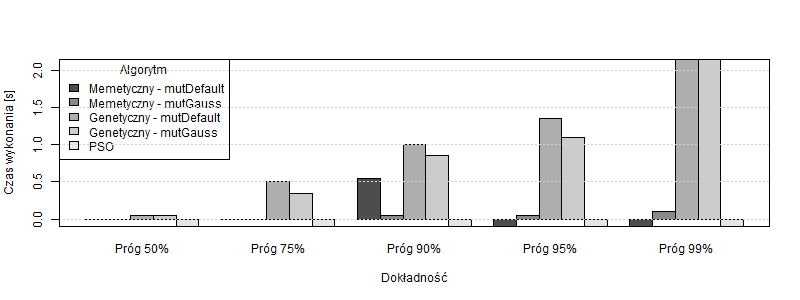
\includegraphics[width=\linewidth]{{img//roz04//kryt2//kryt2_czas_uzyskania_poziomu_dokladnosci_Zeldasine.png}}
  \caption{Wszystkie algorytmy i progi dokładności}
\end{subfigure} 
\begin{subfigure}{\textwidth}
  \centering
  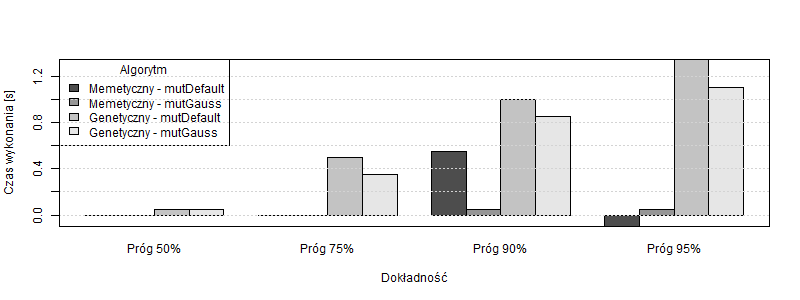
\includegraphics[width=\linewidth]{img//roz04//kryt2//kryt2_czas_uzyskania_poziomu_dokladnosci_bez_PSO_Zeldasine.png}
  \caption{Wszystkie algorytmy i progi dokładności z wyłączeniem PSO i progu 99\%}
\end{subfigure} 
\caption{Czas osiągnięcia rozwiązania o zadanej dokładności - \emph{ZeldaSine10}}
\label{fig:kryt2_Zeldasine}
\end{figure}
%%%%%%%%%%%%%%%%%%%%%%%%%%%%%%%%%%%%%%%%%%



\FloatBarrier
\par
Podsumowując analizę porównawczą w oparciu o \emph{kryterium nr 2}, wnioski pozostają bardzo zbliżone do tych odnośnie \emph{kryterium nr 1}. Mechanizmem uzyskującym bardzo dokładne rozwiązanie w najkrótszym czasie zdecydowanie jest algorytm memetyczny. Porównując operatory mutacji ze sobą w większości przypadków lepsze rezultaty uzyskano wykorzystując \emph{mutGauss} niż \emph{mutDefault}. \emph{PSO} po raz kolejny okazał się najgorszym z badanych algorytmów. 

\subsection{Kryterium nr 3 - powtarzalność skutecznej optymalizacji}
%
%\begin{itemize}
%\item operator mutDefault w porównaniu do mutGauss dla Schaffera wypadł bardzo słabo, dla poziomu 0.01 nawet PSO uzyskało wyższą powtarzalność uzyskania rozwiązania danej dokładności niz algorytmu z mutDefault
%\item ogólnie dla tego kryterium memetyczny wypada najlepiej
%\item w Pavianim zerowe wyniki są konsekwencją znajdowania innego minimum lokalnego o wartości bliskiej optimum. patrz \ref{table:kryt1_Paviani_best_fitness}. 
%\item zeldasine - dziwne ze dla memetycznego mutgauss wyszedl gorzej niz mutdefault
%\item zeldasine - ale dla genetycznego już znacznie lepiej wyszedl mutgauss
%\item PSO bliskie optimum znajduje tylko dla Schaffer, a dla pozostałych nie radzi wcale
%\end{itemize}


\par 
\emph{Kryterium nr 3} porównuje algorytmy optymalizacji na podstawie powtarzalności uzyskiwania rozwiązania bliskiemu optymalnego - nie pod kątem jego wartości, ale euklidesowej odległości w przestrzeni dziedziny możliwych rozwiązań. W przypadku optymalizacji wielomodalnych funkcji to kryterium pozwala określić podatność mechanizmów na utknięcie populacji w lokalnym ekstremum o zbliżonej do optimum wartości.

\par
Analizując wyniki badań porównawczych dla funkcji \emph{Schaffer nr 2} przedstawionych na wykresie \ref{fig:kryt3_Schaffer} ujawnia się przewaga operatora \emph{mutGauss} nad domyślną mutacją. Gaussowska wersja algorytmu memetycznego uzyskała powtarzalność znajdowania rozwiązania o najniższej odległości od optimum na poziomie ponad $60\%$. Następnym pod tym kątem mechanizmem okazał się algorytm genetyczny również wykorzystujący \emph{mutGauss}. W przypadku funkcji \emph{Schaffer nr 2} operator \emph{mutDefault} osiągał gorsze rezulaty nawet od \emph{PSO}, aż do poziomu dokładności $0.01$. Najniższy z badanych poziomów dokładności - $0.015$ - został został osiągnięty przez obie wersje algorytmów memetycznych i genetycznych w prawie wszystkich podjętych próbach. Powtarzalność $97\%$ oznacza, że dla 30 prób testowych tylko raz nie uzyskano rozwiązania o takiej bliskości względem optimum.


%%%%%%%%%%%%%%%%%%%%%%%%%%%%%%%%%%%%%%%%%%%%%%%
\begin{figure}[htb] 
\centering
  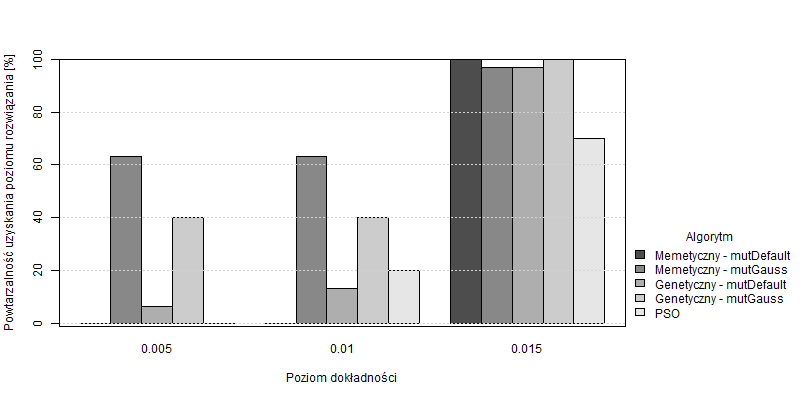
\includegraphics[width=\linewidth]{{img//roz04//kryt3//kryt3_czas_uzyskania_poziomu_dokladnosci_Schaffer.png}}
\caption{Powtarzalność uzyskania rozwiązania o danej dokładności - \emph{Schaffer~nr~2}}
\label{fig:kryt3_Schaffer}
\end{figure}
%%%%%%%%%%%%%%%%%%%%%%%%%%%%%%%%%%%%%%%%%%%%%

\par
Rezultaty dla tego kryterium dla funkcji \emph{Paviani} przedstawiono na wykresie \ref{fig:kryt3_Paviani}. ''Zerowe'' wyniki dla algorytmów innych niż memetyczny można tłumaczyć wynikami uzyskanymi również w badaniach porównawczych wykorzystujących \emph{kryterium nr 1}. W tabeli \ref{table:kryt1_Paviani_best_fitness} przedstawiono dokładne wartości najlepszych znalezionych rozwiązań, z których wynika, że jedynie algorytm memetyczny uzyskał optimum, a algorytm genetyczny inne z lokalnych ekstremów. Bezbłędną skuteczność algorytmu memetycznego w obu wersjach mutacji potwierdza wysoką skuteczność zastosowanej metody lokalnego przeszukania. 

%%%%%%%%%%%%%%%%%%%%%%%%%%%%%%%%%%%%%%%%%%%%%%%
\begin{figure}[hbt] 
\centering
  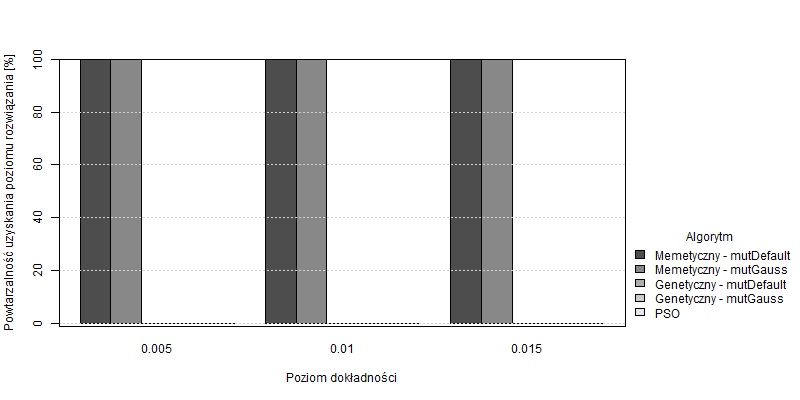
\includegraphics[width=\linewidth]{{img//roz04//kryt3//kryt3_czas_uzyskania_poziomu_dokladnosci_Paviani.png}}
\caption{Powtarzalność uzyskania rozwiązania o danej dokładności - \emph{Paviani}}
\label{fig:kryt3_Paviani}
\end{figure}
%%%%%%%%%%%%%%%%%%%%%%%%%%%%%%%%%%%%%%%%%%%%%

\par
W przypadku ostatniej z testowych funkcji bardzo wysoką skuteczność uzyskał algorytm memetyczny w obu wersjach. Wykorzystując \emph{mutGauss} jedynie w dwóch z trzydziestu prób nie uzyskano rozwiązania bliskiego optimum. Algorytm genetyczny uzyskiwał kolejne poziomy dokładności znacznie rzadziej. Dla tego mechanizmu widoczna jest znaczna przewaga \emph{mutGauss} nad \emph{mutDefault}. Podobnie jak w przypadku \emph{krytetium nr 2}, \emph{PSO} nie uzyskał w żadnej z prób rozwiązania wystarczająco bliskiego by zaliczać się choćby do najniższej badanej dokładności. Dokładne wyniki dla \emph{ZeldaSine10} przedstawiono na wykresie \ref{fig:kryt3_Zeldasine}.

%%%%%%%%%%%%%%%%%%%%%%%%%%%%%%%%%%%%%%%%%%%%%%%
\begin{figure}[hbt] 
\centering
  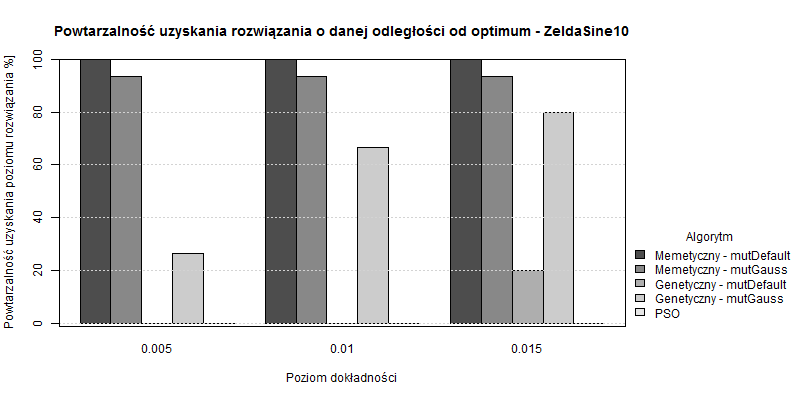
\includegraphics[width=\linewidth]{{img//roz04//kryt3//kryt3_czas_uzyskania_poziomu_dokladnosci_Zeldasine.png}}
\caption{Powtarzalność uzyskania rozwiązania o danej dokładności - \emph{ZeldaSine10}}
\label{fig:kryt3_Zeldasine}
\end{figure}
%%%%%%%%%%%%%%%%%%%%%%%%%%%%%%%%%%%%%%%%%%%%%

\FloatBarrier


\subsection{Kryterium nr 4 - ogólna charakterystyka populacji}

\par
Ostatnie z przyjętych w analizie porównawczej kryteriów opisuje jak zmienia się różnorodność populacji opisywana poprzez różnicę między najlepszym i średnim rozwiązaniem danej iteracji wszystkich osobników. Wartość średniego rozwiązania populacji może się różnie zmieniać w zależności od specyfiki rozpatrywanego problemu. W przypadku funkcji \emph{Schaffer nr 2} w przyjętym okresie 100 iteracji algorytmów utrzymuje się na stałym poziomie około $0.5$, co jest konsekwencją faktu, że większość dziedziny rozwiązań koduje wartości bliskie $0.5$, a większe różnice znajdują się jedynie w wąskim sąsiedztwie poszukiwanego optimum. Przebieg kryteriów dla pozostałych funkcji jest bardziej zróżnicowany - średnie rozwiązanie populacji stopniowo zbliża się do wartości optymalnej. Zgodną cechą dla wszystkich algorytmów i funkcji testowych jest największa dynamika zmian różnic w pierwszych 20 iteracjach. Pokrywa się to z obserwacją najefektywniejszej optymalizacji na początku działania algorytmów. 
\par
W przypadku funkcji \emph{Schaffer nr 2}, wszystkie algorytmy uzyskały bardzo zbliżone rezultaty dla tego kryterium. Wynik jest zgodny z obserwacją dla \emph{kryterium nr 1}, gdzie każdy algorytm uzyskiwał rezultaty bardzo bliskie wartości optymalnej. Płaski przebieg wykorzystanej funkcji powoduje niezmienność średniego rozwiązania populacji w trakcie działania algorytmu. Na wykresie \ref{fig:kryt4_Schaffer} przedstawiono komplet uzyskanych wyników badań porównawczych. 
%
%\begin{itemize}
%\item dla Schaffera wszystkie algorytmy zachowują się bardzo podobnie - ogół populacji rozklada sie w szerokiej plaskiej czesci przebiegu funkcji, a najlepsze osobniki już w 10 iteracjach zblizają się do optimum
%\item dla Paviani - różnica w 10 iteracja szybko spada, co oznacza, że i
%\item dla Paviani - mutgauss osiaga nizsze roznice zarowno dla memetycznego i genetcznego niz mutdefault
%\item dla Zeldasine - mutDefault osiaga wyzsze roznice niz mutGauss
%\end{itemize}
%%%%%%%%%%%%%%%%%%%%%%%%%%%%%%%%%%%%%%%%%%%%%%%
\begin{figure}[hbt] 
\centering
  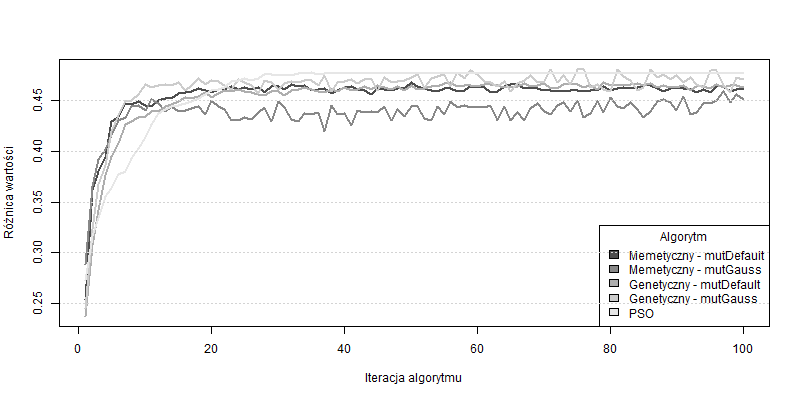
\includegraphics[width=\linewidth]{{img//roz04//kryt4//kryt4_czas_uzyskania_poziomu_dokladnosci_Schaffer.png}}
\caption{Różnica pomiędzy średnim i najlepszym rozwiązaniem populacji w kolejnych iteracjach algorytmu - \emph{Schaffer~nr~2}}
\label{fig:kryt4_Schaffer}
\end{figure}
%%%%%%%%%%%%%%%%%%%%%%%%%%%%%%%%%%%%%%%%%%%%%

\par
W przypadku funkcji \emph{Paviani} uwidacznia się różnica pomiędzy zastosowanymi operatorami mutacji. Zarówno algorytm memetyczny jak i genetyczny wykorzystujący \emph{mutGauss} po około 20 iteracjach doprowadza średnie rozwiązania populacji blisko do poziomu obecnie najlepszego osobnika. Porównując mechanizmy wykorzystujące \emph{mutDefault} niższą różnicę osiąga memetyczny. Algorytm \emph{PSO}, po początkowych dynamicznych zmianach różnicy, stabilizuje się na poziomie podobnym do genetycznego z domyślną mutacją. Przebieg zmian różnic dla wszystkich algorytmów przedstawiono na wykresie \ref{fig:kryt4_Paviani}.

%%%%%%%%%%%%%%%%%%%%%%%%%%%%%%%%%%%%%%%%%%%%%%%
\begin{figure}[hbt] 
\centering
  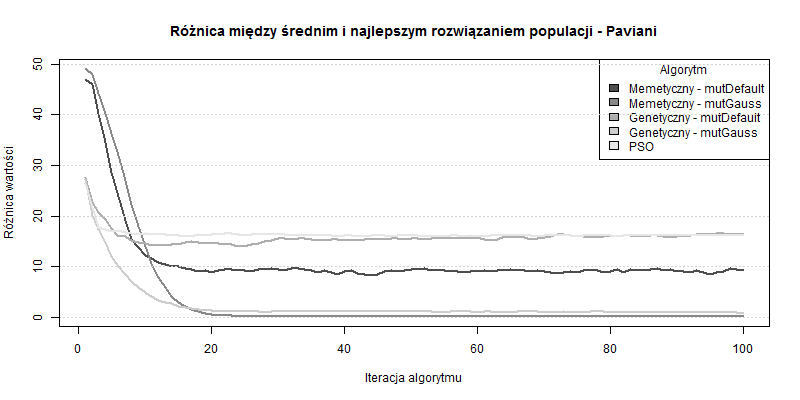
\includegraphics[width=\linewidth]{{img//roz04//kryt4//kryt4_czas_uzyskania_poziomu_dokladnosci_Paviani.png}}
\caption{Różnica pomiędzy średnim i najlepszym rozwiązaniem populacji w kolejnych iteracjach algorytmu  - \emph{Paviani}}
\label{fig:kryt4_Paviani}
\end{figure}
%%%%%%%%%%%%%%%%%%%%%%%%%%%%%%%%%%%%%%%%%%%%%

Wyniki badań \emph{kryterium nr 4} dla ostatniej funkcji testowej przedstawiono na wykresie \ref{fig:kryt4_Zeldasine}. Podobnie jak w przypadku \emph{Paviani} algorytmy wykorzystujące gaussowską mutację po około 20 iteracjach uzyskują średnie rozwiąznie bliskie najlepszemu. Mechanizmy oparte na \emph{mutDefault} w trakcie działania stabilizują różnicę na tym samym poziomie, nawet pomimo tego, że początkowo ich przebiegi znacznie się różnią. W przypadku algorytmu \emph{PSO} dystans pomiędzy średnim i najlepszym rozwiązaniem mieści się pomiędzy rezultatami dla \emph{mutDefulat} i \emph{mutGauss}.

%%%%%%%%%%%%%%%%%%%%%%%%%%%%%%%%%%%%%%%%%%%%%%%
\begin{figure}[hbt]
\centering
  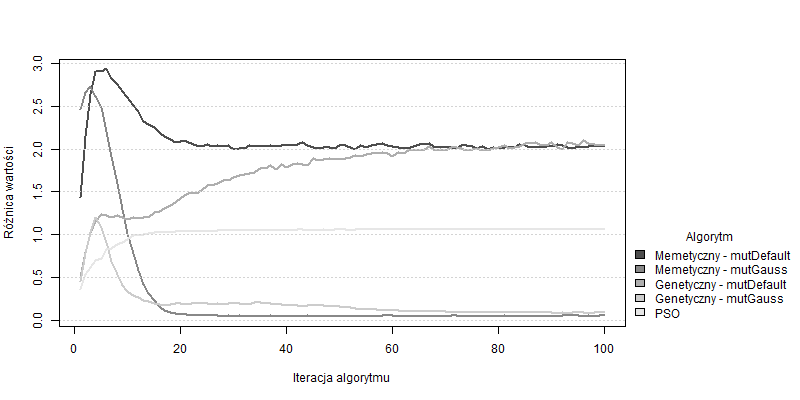
\includegraphics[width=\linewidth]{{img//roz04//kryt4//kryt4_czas_uzyskania_poziomu_dokladnosci_Zeldasine.png}}
\caption{Różnica pomiędzy średnim i najlepszym rozwiązaniem populacji w kolejnych iteracjach algorytmu  - \emph{ZeldaSine10}}
\label{fig:kryt4_Zeldasine}
\end{figure}
%%%%%%%%%%%%%%%%%%%%%%%%%%%%%%%%%%%%%%%%%%%%%
\FloatBarrier

\par
Podsumowując wyniki uzyskane w badaniach dla tego kryterium, największy wpływ na różnorodność populacji ma zastosowany operator mutacji. Jest to konsekwencją logiki jego działania - \emph{mutDefault} losuje nową wartość atrybutu z pełnego zakresu jego dziedziny, zaś mutacja gaussowska znajduje nową wartość w najbliższym otoczeniu dotychczasowej wartości. Algorytm \emph{PSO} osiąga niższą różnicę między najlepszym i średnim rozwiązaniem, jednakże należy zaznaczyć, że dla funkcji \emph{Paviani} i \emph{ZeldaSine10} mechanizm ten nie jest w stanie znaleźć rozwiązania bliskiemu optymalnego. 
\newpage
\chapter{Wnioski i podsumowanie}
\begin{itemize}
%\item Analiza porównawcza:
%\begin{itemize}
%\item dla kryt nr 1 - algorytm memetyczny i genetyczny uzyskał bardzo podobne rozwiązania, ale memetyczny znacznie szybciej
%\item dla kryt nr 1 - mutGauss opóźnił stagnację memetycznego i przyspieszył genetycznego
%\item dla kryt nr 1 - PSO dużo gorszy od pozostałych
%\item dla kryt nr 2 - memetyczny z mutGauss najszybciej osiągnął kolejne progi progi
%\item dla kryt nr 2 - mutGauss wyraźnie lepszy od mutDefault
%\item dla kryt nr 2 - PSO dużo gorszy
%\item dla kryt nr 3 - memetyczny z mutGauss zdecydowanie najlepszy dla Schaffer nr 2, dla pozostałych równy z memetycznym z mutDefault
%\item dla kryt nr 3 - mutGauss lepszy niż mutDefault
%\item dla kryt nr 4 - największy wpływ na różnicę ma operator mutacji
%\item dla kryt nr 4 - mem i gen z tymi samymi operatorami osiągaja bardzo podobne rezultaty
%\item dla kryt nr 4 - największa dynamika zmian różnicy jest w pierwszych 20 iteracjach
%
%\item
%\end{itemize} 
\item Dobór parametrów:
\begin{itemize}
\item dla funkcji trudnooptymalizowanych najlepsze konfiguracje uzyskano scenariuszami dobierającymi trójkami
\item nieznacznie gorsze okazał sie scenariusz [3-6, 1-2, 4-5]
\item dobieranie dwójkami jest znacznie szybsze
\item mutGauss uzyskuje lepsze rezultaty, ale proces selekcji jest wolniejszy
\end{itemize}
\item powstała aplikacja umożliwia powtórzenie i przeprowadzenie kolejnych badan
\end{itemize}

\par
Analizując wyniki uzyskane w trakcie badań porównawczych można dojść do wniosku, że algorytm memetyczny stanowi znacznie lepszą metodę rozwiązywania rzeczywistoliczbowych problemów optymalizacyjnych. Prawie dla każdego z wykorzystanych kryteriów uzyskał znacznie lepsze rezultaty niż pozostałe algorytmy wykorzystane do porównania. Ostateczne podsumowanie rezultatów uzyskanych dla użytych kryteriów rozpatrując głównie różnice pomiędzy wykorzystywanymi algorytmami przedstawia się następująco:
\begin{itemize}
\item kryterium nr 1 wykazało, że zarówno algorytm memetyczny jak i genetyczny uzyskuje bardzo podobne, bliskie optimum rozwiązania, ale memetyczny dokonuje tego szybciej, 
\item kryterium nr 2 wykazało, że algorytm memetyczny wykorzystujący mutację \emph{mutGauss} najszybciej osiągnął kolejne progi jakości rozwiązania, 
\item kryterium nr 3 wykazało przewagę w powtarzalności uzyskiwania rezultatów bliskich optimum nad algorytmem genetycznym i \emph{PSO},
\item kryterium nr 4 nie wykazało większej zależności pomiędzy użytym algorytmem, a różnicą pomiędzy najlepszym i średnim rozwiązaniem w populacji - wpływ na ten aspekt ma wykorzystany operator mutacji.
\end{itemize}

\par 
Przeprowadzenie badań z wykorzystaniem dwóch wersji operatora mutacji pozwoliło na przeprowadzenie analizy różnicy w ich skuteczności. W ogólnym rozrachunku lepsze rezultaty uzyskano z wykorzystaniem \emph{mutGauss}. Kosztem uzyskania wyższych wyników przy wykorzystaniu tego operatora jest jednak dłuższy czas działania pojedynczej iteracji algorytmu. Może to być jednakże konsekwencja nieoptymalnej własnej implementacji spowodowanej niewystarczającą biegłością autora pracy w posługiwaniu się językiem \emph{R}. Zebranie wniosków dotyczących porównania dwóch wykorzystanych operatorów mutacji można opisano poniżej:
\begin{itemize}
\item kryterium nr 1 wskazało na to, że użycie \emph{mutGauss} przyspiesza stagnację populacji algorytmu memetycznego, ale opóźnia w przypadku algorytmu genetycznego,
\item kryterium nr 2 wykazało zdecydowaną przewagę operatora \emph{mutGauss} nad \emph{mutDefault} jeśli chodzi o szybkość osiągania poszczególnych progów jakości rozwiązania
\item kryterium nr 3 wskazało na to, że mutacja gaussowska umożliwie z większą powtarzalnością uzyskanie rozwiązania bliskiego optimum,
\item kryterium nr 4 wykazało, że zastosowanie domyślnego operatora mutacji znacznie zwiększa różnorodność genetyczna populacji, czego oznaką jest większa różnica pomiędzy najlepszym i średnim rozwiązaniem populacji.
\end{itemize}

\par
Pełne podsumowanie badań porównawczych przedstawiono w tabeli \ref{table:wnioski_zestawienie_wynikow}. Znakiem $+$ oznaczono tam, który z algorytmów i operatorów uzyskał najlepsze rezultaty dla danego kryterium i funkcji testowej. Oznaczenie dwóch algorytmów lub mechanizmów mutacji dla jednego kryterium jest konsekwencją uzyskania tych samych wyników przez więcej niż jedną badaną konfigurację. Ostatni wiersz tabeli przedstawiający sumę \emph{zwycięstw} poszczególnych opcji ostatecznie potwierdza przewagę algorytmu memetycznego nad pozostałymi wykorzystanymi w analizie porównawczej. Niewielka różnica w wynikach dla operatorów mutacji spowodowana jest faktem, że dla wielu kryteriów wyniki uzyskane obydwoma były takie same, przypadki zwycięstwa \emph{mutDefault} uzyskane zostały przy niewielkiej różnicy względem \emph{mutGauss}, zaś każda z sytuacji dominacji gaussowskiego mechanizmu mutowania osobników odznaczała się zdecydowaną przewagą nad domyślnym algorytmem pakietu \emph{GA}.
 

\newcolumntype{?}{@{\hskip\tabcolsep\vrule width 1pt\hskip\tabcolsep}}

\begin{table}[hbt]
\caption{Zestawienie wyników badań dla kryteriów porównawczych}
\label{table:wnioski_zestawienie_wynikow}
\begin{center}
\begin{tabularwithnotes}{|c|l?c|c|c?c|c|}
{
  \tnote[1]{\emph{Algorytm memetyczny}}
  \tnote[2]{\emph{Algorytm genetyczny}}
 }
	\Xhline{1pt}
	\multirow{2}{*}{Funkcja} & \multicolumn{1}{c?}{\multirow{2}{*}{Kryterium}} & \multicolumn{3}{c?}{Algorytm} & \multicolumn{2}{c|}{Operator mutacji} \\
	\cline{3-7}	
	{} & {} & \emph{mem}\tmark[1] & \emph{gen}\tmark[2] & \emph{PSO} & \emph{mutGauss} & \emph{mutDefault} \\
	\Xhline{1pt}	
	\multirow{8}{*}{\emph{Schaffer nr 2}} & Kr. 1 - rozwiązanie &+ & & &+ & \\ \cline{2-7}
	{} & Kr. 1 - stagnacja &+ & & & &+ \\ \cline{2-7}
	{} & Kr. 2 - próg 99\% &+ & & &+ & \\ \cline{2-7}
	{} & Kr. 2 - próg 95\% & &+ & &+ & \\ \cline{2-7}
	{} & Kr. 3 - dokładność 0.005 &+ & & &+ & \\ \cline{2-7}
	{} & Kr. 3 - dokładność 0.01 &+ & & &+ & \\ \cline{2-7}
	{} & Kr. 4 - różnica po 10 it. & &+ & &+ & \\ \cline{2-7}
	{} & Kr. 4 - różnica po 100 it. & & &+ &+ & \\
	\Xhline{1pt}
	\multirow{8}{*}{\emph{Paviani}} & Kr. 1 - rozwiązanie &+ & & &+ &+ \\ \cline{2-7}
	{} & Kr. 1 - stagnacja &+ & & & &+ \\  \cline{2-7}
	{} & Kr. 2 - próg 99\% &+ & & &+ &+ \\ \cline{2-7}
	{} & Kr. 2 - próg 95\% &+ & & &+ &+ \\ \cline{2-7}
	{} & Kr. 3 - dokładność 0.005 &+ & & &+ &+ \\ \cline{2-7}
	{} & Kr. 3 - dokładność 0.01 &+ & & &+ &+ \\ \cline{2-7}
	{} & Kr. 4 - różnica po 10 it. &+ & & &+ & \\ \cline{2-7}
	{} & Kr. 4 - różnica po 100 it. & &+ &+ & &+ \\
	\Xhline{1pt}
	\multirow{8}{*}{\emph{ZeldaSine10}} & Kr. 1 - rozwiązanie &+ &+ & &+ &+ \\ \cline{2-7}
	{} & Kr. 1 - stagnacja &+ & & & &+ \\ \cline{2-7}
	{} & Kr. 2 - próg 99\% &+ & & &+ & \\ \cline{2-7}
	{} & Kr. 2 - próg 95\% &+ & & &+ & \\ \cline{2-7}
	{} & Kr. 3 - dokładność 0.005 &+ & & & &+ \\ \cline{2-7}
	{} & Kr. 3 - dokładność 0.01 &+ & & & &+ \\ \cline{2-7}
	{} & Kr. 4 - różnica po 10 it. &+ & & & &+ \\ \cline{2-7}
	{} & Kr. 4 - różnica po 100 it. &+ &+ & & &+ \\
	\Xhline{1pt}
	\multicolumn{2}{|c?}{Suma} & 20 & 5 & 2 & 16 & 14 \\
	\Xhline{1pt}
\end{tabularwithnotes}
\end{center}
\end{table}





%\bibliographystyle{plalpha}
\bibliographystyle{plabbrv}

%UWAGA: bibliotekę referencji należy przygotować samemu. Dobrym do tego narzędziem jest JabRef.
%       Nazwę przygotowanej biblioteki wpisuje się poniżej bez rozszerzenia 
%       (w tym przypadku jest to "dokumentacja.bib")
\bibliography{bibtex}

\appendix
\chapter{Aplikacja - symulator}
\section{Założenia projektowe aplikacji}
\section{Instrukcja instalacyjna}
\section{Opis interfejsu graficznego}


\end{document}
